\documentclass[conference]{IEEEtran}
%\IEEEoverridecommandlockouts
% The preceding line is only needed to identify funding in the first footnote. If that is unneeded, please comment it out.


%%%%%%%%%%%%%%%%%%%%%%%%%%%%%%%%%%%%%%%%%%%%%%%%%%%%%%%%%%%%%%%%%%%%%%%%%%%%%%

%% Beautiful mathematics
\usepackage{amsmath, amssymb, amsfonts} 
\usepackage{nicefrac}
\usepackage{mathtools}
\usepackage{bm, bbm}
\usepackage[scr=boondoxo,scrscaled=1.05]{mathalfa}

%% References in the correct format 
%\usepackage[square,numbers]{natbib}
%\def\bibfont{\footnotesize} % fix to have the same font size as without natbib

\usepackage[sort, compress, space]{cite}            


%% Enumerate nicely 
\usepackage{enumitem}

%% Different color comments and commenting large parts of the text
\usepackage{xcolor}
\usepackage{comment}
\usepackage{soul}

%% Hyper references
\usepackage{hyperref}
\usepackage{cleveref}
%\usepackage[numbers]{natbib}

\usepackage{tikz}
%\usepackage{thm-restate}
%% Appendix package
%\usepackage{appendix}

%% Random text to test spacing 
\usepackage{blindtext}

\usepackage{afterpage}

\usepackage{algorithm, algorithmic}    



\usepackage{dsfont}

\usepackage{tikz}
\usepackage{graphicx}
\usepackage{tikzscale}
\usepackage{pgfplots}
\pgfplotsset{compat=newest}
\usepackage{xfrac}

\usepackage{thm-restate}

%\usepackage{subcaption}

\usepackage{balance}

\usepackage{cite}
\usepackage{amsmath,amssymb,amsfonts}
\usepackage{balance}
\usepackage{algorithmic}
\usepackage{graphicx}
\usepackage{textcomp}
\usepackage{xcolor}
\usepackage{amsmath}
\usepackage{amssymb}
\usepackage[mathscr]{euscript}
\usepackage{comment}
\usepackage{xcolor}
\usepackage{enumitem} 
\usepackage{amsthm}







\begin{document}


\title{Order Fairness Evaluation of DAG-based ledgers}


\author{\IEEEauthorblockN{Erwan Mahe \orcidlink{0000-0002-5322-4337}}
\IEEEauthorblockA{\textit{Université Paris Saclay, CEA LIST} \\
Palaiseau, France}
\and
\IEEEauthorblockN{Sara Tucci-Piergiovanni \orcidlink{0000-0001-9738-9021}}
\IEEEauthorblockA{\textit{Université Paris Saclay, CEA LIST} \\
Palaiseau, France}
}

\maketitle

\begin{abstract}
In Distributed Ledgers (DL), Order Fairness (OF) refers to properties that relate the order in which transactions are sent or received to the order in which they are eventually finalized (totally ordered). 
The study of OF is relatively new and has been stimulated by the rise of Maximal Extractable Value attacks.
In classical Blockchain protocols, leaders are responsible for selecting the transactions to be included in blocks, which creates a vulnerability and opportunity for transaction order manipulation.
Unlike Blockchains, DAG-based DL allow participants in the network to independently propose blocks, which are then arranged as vertices of a directed acyclic graph. Interestingly, leaders in DAG-based ledgers are elected only \textit{après coup} (after the fact), once transactions are already part of the graph, to determine their total order. In other words, transactions are collectively validated by the nodes, and leaders are only elected to establish an ordering. This approach intuitively reduces the risk of transaction manipulation and enhances fairness.

In this paper, we aim to quantify the capability of DAG-based DL to achieve OF. To this end, we define new variants of OF adapted to DAG-based DL and evaluate the impact of an adversary capable of compromising a limited number of nodes (below the one-third threshold) to reorder transactions. We analyze how often our OF properties are violated under different network conditions and parameterizations of the DAG algorithm, depending on the adversary’s power.
Our study shows that DAG-based DL are still vulnerable to reordering attacks, as an adversary can coordinate a minority of Byzantine nodes to manipulate the DAG's structure.
\end{abstract}





\begin{IEEEkeywords}
DAG-based Distributed Ledger,
Transaction Ordering,
Order Fairness
\end{IEEEkeywords}






\section{Introduction}
\label{sec:intro}
% Image editing methods in diffusion models depend on user-defined control directions - users can unlock their creativity using these methods by specifying the desired manipulation through prompts~\cite{gandikota2023concept}, reference images~\cite{ruiz2022dreambooth, kumari2022customdiffusion, gal2022image, chen2024trainingfreeregionalpromptingdiffusion}, or attribute vectors~\cite{parmar2023zero,hertz2022prompt}. In this work, we ask a fundamentally different question: \emph{Can we automatically discover the underlying visual structure of a concept within diffusion model's knowledge?} %Rather than requiring user-specified controls, we aim to decompose the model's internal knowledge into meaningful directions.

% This question touches on a fundamental limitation in how we interact with diffusion models. Current control methods ~\cite{zhang2023addingconditionalcontroltexttoimage, gandikota2023concept, ye2023ipadaptertextcompatibleimage,ye2023ipadaptertextcompatibleimage, hertz2024stylealignedimagegeneration, li2023photomaker, shi2024instantbooth, chen2024trainingfreeregionalpromptingdiffusion} require users to specify their desired manipulations in advance, limiting interactive creativity. This contrasts with natural human artistic workflows, where creators dynamically explore creative ideas while jointly refining them toward meaningful artistic outcomes~\cite{hoffmann2016modeling}. This synergy between specification and exploration is not new to generative models. Early GAN architectures naturally developed disentangled latent spaces that enabled continuous\cite{harkonen2020ganspace,radford2015unsupervised, wu2021stylespace, shen2020interfacegan}, compositional control over generated images. Users could explore these spaces to discover interesting variations that would be difficult to describe in words~\cite{wu2021stylespace}, then combine them to achieve their creative goals~\cite{grabe2022towards}. 


% While diffusion models have largely superseded GANs in conditional image synthesis~\cite{dhariwal2021diffusion},  their underlying structure remains less understood. Diffusion models achieve remarkable diversity through high-dimensional latents, unlike GANs' compact latent spaces.  With a single prompt, diffusion models can generate radically different variations through different random initializations of input noise. We ask - Is it possible to discover interpretable structure within this vast space of variations?

Text-to-image diffusion models are capable of generating remarkable visual variations from a single prompt through different random initializations. However, this vast creative potential remains largely opaque to users---while we can generate diverse images, we lack understanding of the underlying structure of these variations. This presents a fundamental challenge: how can we discover and expose the latent visual capabilities encoded within these models?

\let\thefootnote\relax \footnote{$^{*}$Correspondence to \texttt{gandikota.ro@northeastern.edu}}

The challenge touches on a key limitation in how we interact with diffusion models today. Current control methods require users to explicitly specify their desired edits in advance through prompts~\cite{gandikota2023concept}, reference images~\cite{zhang2023addingconditionalcontroltexttoimage, chen2024trainingfreeregionalpromptingdiffusion, ruiz2022dreambooth,kumari2022customdiffusion, Ryu_lora, hu2021lora}, or attribute vectors~\cite{ye2023ipadaptertextcompatibleimage, hertz2024stylealignedimagegeneration, li2023photomaker, shi2024instantbooth,parmar2023zero,hertz2022prompt}. That contrasts sharply with natural human creative workflows, where artists dynamically explore creative ideas and jointly refine them toward meaningful artistic outcomes~\cite{hoffmann2016modeling}. The need for pre-specified controls creates a barrier between users and the full creative potential of these models.

Interestingly, earlier generative models like GANs~\cite{gans,karras2019style,brock2018large} naturally developed more interpretable internal structures. Their compact latent spaces often exhibited emergent disentanglement~\cite{harkonen2020ganspace,radford2015unsupervised, wu2021stylespace, shen2020interfacegan}, enabling continuous and compositional control over generated images. Users could explore these spaces to discover interesting variations that would be difficult to describe in words~\cite{wu2021stylespace}, then combine them to achieve their creative goals~\cite{grabe2022towards}.

Diffusion models have largely superseded GANs in conditional image synthesis~\cite{dhariwal2021diffusion}, achieving greater diversity through much higher-dimensional latents. And yet an understanding of the underlying structure of these larger latent spaces has remained elusive. In this work, we ask a fundamental question: \emph{Can we automatically discover the visual structure within a diffusion model's knowledge of a concept?} Rather than requiring user-specified controls, we aim to decompose the model's internal representations into expressive directions that users can explore and combine.

To address these needs, we present \textbf{SliderSpace}, a framework that brings systematic explorability to diffusion models. Given just a text prompt, SliderSpace discovers a canonical set of meaningful, diverse, and controllable directions within the model's knowledge of that concept. Each direction is implemented as a low-rank adapter~\cite{hu2021lora} that can be scaled and composed with others, allowing users to explore and smoothly combine different aspects of variation, as shown in Figure~\ref{fig:intro}.

We ground SliderSpace discovery in three key requirements for meaningful decomposition of a diffusion model's visual manifold: 
\begin{enumerate}
    \item \textbf{Unsupervised Discovery:} The decomposition process should emerge from the intrinsic structure of the model's learned representation, rather than being guided by predefined attributes. This ensures we capture the true topology of the model's knowledge space rather than projecting our assumptions onto it.
    
    \item \textbf{Semantic Orthogonality:} Each discovered control must represent a distinct semantic direction. This is enforced in a semantic feature space, like CLIP, where every slider has an orthogonal effect in embeddings. This prevents discovering multiple controls that create similar semantic effects, making the system more efficient and easier.
    
    \item \textbf{Distribution Consistency:} Directions must induce consistent transformations across both random seeds and prompt variations. 
\end{enumerate}

These requirements naturally lead to our proposed framework, which we formalize in Section~\ref{sec:method}. As we show in our experiments, SliderSpace is architecture-agnostic, working with both conventional U-Net based models like Stable Diffusion~\cite{rombach2022high, rombach2022sd20, podell2023sdxl, turbo, dmd} and recent transformer-based architectures like Flux~\cite{flux}.

We demonstrate the expressiveness of SliderSpace through three applications: First, we show how SliderSpace can decompose high-level concepts into diverse and expressive components, revealing the natural axes of variation in the model's understanding. Second, we explore artistic style variation, where SliderSpace discovers directions that match or exceed the diversity of manually curated artist lists while being judged more useful by human evaluators. Finally, we show how SliderSpace can help reverse the mode collapse commonly observed in distilled diffusion models, restoring diversity while maintaining generation speed.

Beyond providing practical creative control, SliderSpace opens new avenues for understanding and utilizing the latent capabilities of diffusion models. By mapping these models' visual potential into intuitive, composable directions, we take a step toward making their creative possibilities more accessible and interpretable to users.

% Image editing methods in diffusion models unlock the creativity of users. In this work we ask an alternate question: \emph{Can we organize and expose what of the diffusion model is already capable of?}.
% Existing methods for controlling image generation typically require users to manually specify edit directions for desired changes. This process is time-consuming, requires technical expertise, and limits the spontaneity of the creative process. For instance, if a user wants to adjust the smile of a generated person, they must explicitly request this edit, often through imprecise prompt engineering or model fine-tuning. This approach of predefined controls or manual specifications restricts users from fully exploring the latent capabilities of the model. There may be interesting stylistic variations or attributes that the model can generate, but users have no easy way to discover or utilize these.

% Natural visual disentanglement was an emergent property in the latent space of Generative Adversarial Models (GANs) \cite{harkonen2020ganspace,radford2015unsupervised, wu2021stylespace, shen2020interfacegan}. In particular, it has been observed that StyleGAN~\cite{karras2019style} stylespace neurons offer detailed control over many meaningful aspects of images that would be difficult to describe in words~\cite{wu2021stylespace}. However, diffusion models do not share such a compact latent space~\cite{park2023unsupervised}; and efforts to uncover such a space in the semantic embeddings of the text conditioning have met with limited success \nik{Nick - is there a specific citation you were thinking about?}.

% In this work we introduce \textbf{SliderSpace}, which takes a step towards uncovering an analogous low dimensional representation of diffusion models' visual breadth; in essence treating the diffusion model as many generators sharing parameters, where a particular generator is defined by a specific prompt. For a given prompt we sample many random seeds (and optionally prompt expansions using an LLM), generate the corresponding images, and apply an off the shelf feature extractor (in this work CLIP, but our method can be applied to any differentiable feature extractor). We use PCA to analyze these features, and for each of the leading $k$ principal components we train a LoRA \cite{} which causes the diffusion model to produces images which increase the feature magnitude along that component when passed back through the same feature extractor. This leads to a 'Slider' for each principal component, because each LoRA can be scaled and applied to the original diffusion model, continuously varying those visual features in the generated results (as measured, in our case, by CLIP).

% There are many other works that enhance the controllability of diffusion models. One common approach is enabling users to add spatial constraints to a generation either manually, or via a reference image \cite{zhang2023addingconditionalcontroltexttoimage, chen2024trainingfreeregionalpromptingdiffusion}, a second is leveraging more abstract embeddings (e.g. identity, style) extracted from a reference image \cite{ye2023ipadaptertextcompatibleimage, hertz2024stylealignedimagegeneration, li2023photomaker, shi2024instantbooth}, a third is finetuning a foundation model to better generate a concept important to the user \cite{ruiz2022dreambooth, kumari2022customdiffusion, Ryu_lora, hu2021lora}, and a fourth (most relevant to this work) is finding low-rank adaptors of the model based on a prompt or small training set which can be scaled to provide continous control over one aspect of generated image (e.g. night vs day, basic vs luxury, etc.) \cite{gandikota2023concept}. SliderSpace is complementary to all of these methods and offers something distinct. All of the other methods we are aware require the user (and / or model designer) to know in advance what type of control they want. In contrast SliderSpace assists users in discovering and controlling hidden capabilities present in the diffusion model's distribution of possible generations.

%We propose that truly intuitive creative control in a text-to-image model should meet three key criteria: \emph{discoverability}, \emph{intuitiveness}, and \emph{specificity}. The model should reveal controllable attributes that may not be immediately obvious, offer controls that are easy to understand and manipulate, and ensure each control affects a distinct attribute of the generated image.

% We demonstrate the utility and power of SliderSpace using three applications built on top of SDXL-DMD \cite{dmd}, because its fast generation speed lends itself well to the continuous control offered by SliderSpace.

% First, we study concept decomposition (Section \ref{sec:concept_exp}), where we learn sliders for a specific concept (e.g. 'monster', 'waterfall', 'car'). Through quantitative metrics of diversity and text alignment we demonstrate that the learned sliders dramatically boost the diversity of generations when randomly applied without harming text alignment; we also ask humans to qualitatively judge these results in a user study where they find the SliderSpace results to be more 'Diverse', 'Useful', and 'Creative' than our baselines.

% Second, we attempt to compare the automatic discoveries of SliderSpace to a large scale manual study of artistic styles (Section \ref{sec:art_exp}), open-sourced by ParrotZone \cite{parrotzone}. In this study SDXL was prompted with over 4300 artist names,  and based on visual inspection the cases of successful stylistic mimicry recorded. Quantitatively SliderSpace more closely matches the distribution of artistic variation discovered by ParrotZone than other baselines, and in our user studies was judged to be significantly more 'Diverse' and 'Useful' than the baselines. To our surprise humans even judged SliderSpace results to be slightly more 'Diverse' than the results generated by the manually discovered artist names of \cite{parrotzone}.

% Third, we attempt to use SliderSpace to reverse the mode collapse commonly observed in distilled few-step diffusion models relative to the original teacher model (Section \ref{sec:diverse_exp}). We quantitatively demonstrate that applying SliderSpace to SDXL-DMD leads to more closely matching the distribution of images by the original teacher, SDXL.

%Through extensive experiments on various state-of-the-art text-to-image models, we demonstrate that SliderSpace significantly enhances user control and creative expression in AI-assisted image generation tasks. Our method enables a range of applications, including concept decomposition and control, diversity improvement in generated images, customization dissection and edits, and the exploration of artistic styles inherent in the model.

% SliderSpace goes beyond providing a practical tool for enhanced creative control. By mapping the visual potential of diffusion models it can open new avenues for generative creativity and deepens our understanding of each model's hidden potential.



\section{Preliminaries and related works\label{sec:related}}


Fairness, in the context of Blockchains \cite{on_fairness_in_commitee_based_blockchains,on_fairness_in_voting_consensus_protocols} and DAGs \cite{fairness_notions_in_dag_based_dlts} may refer to various notions, including the fairness in committee selection \cite{on_fairness_in_commitee_based_blockchains}, rewarding \cite{do_the_rich_get_richer_fairness_analysis_for_blockchain_incentives} or the ability to take decisions \cite{on_fairness_in_voting_consensus_protocols,fairledger_a_fair_blockchain_protocol_for_financial_institutions} w.r.t.~individual nodes' voting power. 
While \cite{fairness_and_efficiency_in_dag_based_cryptocurrencies} studies reward fairness in PoW DAGs, \cite{on_fairness_in_voting_consensus_protocols} deals with fairness to validators.
\cite{fairness_notions_in_dag_based_dlts} reviews notions of fairness applied to DAG-based DL.
In \cite{sok_preventing_transaction_reordering_manipulations_in_decentralized_finance} ``fairness'' is achieved whenever participants cannot include, exclude or front-run \cite{flash_boys_frontrunning_in_decentralized_exchanges_miner_extractable_value_and_consensus_instability} a transaction after having seen its content.


In this paper, we are specifically interested in {\em order-fairness} \cite{order_fairness_for_byzantine_consensus,quick_order_fairness,byzantine_ordered_consensus_without_byzantine_oligarchy,themis_fast_strong_order_fairness_in_byzantine_consensus} (OF) properties, that relate partial orders on transaction finalization and on communication events.
\cite{order_fairness_for_byzantine_consensus} defines ``\textit{receive-order fairness}'' as follows: if a majority of nodes receive a transaction $x$ before $x'$ then $x$ must be finalized before $x'$.
However, for three transactions $x_1$, $x_2$ and $x_3$, it may be so that a majority of nodes receive $x_1$ before $x_2$, $x_2$ before $x_3$ and $x_3$ before $x_1$. Thus, this property is impossible to achieve, as $\{x_1,x_2,x_3\}$ forms a Condorcet cycle \cite{condorcet_attack_against_fair_transaction_ordering}.
As a solution, \cite{quick_order_fairness} proposes the achievable ``\textit{differential-order fairness}'', which rather considers the difference between the number of honest nodes that receive $x$, and resp.~$x'$ first.
%If this differences exceeds $2*f$, then $x$ must be finalized before $x'$.
\cite{themis_fast_strong_order_fairness_in_byzantine_consensus} proposes ``\textit{$\gamma$-(all)-batch-order fairness}'' that reasons on pairs of transactions that are not in the same Condorcet cycle.
%as follows: for $\gamma \geq 1/2$, if a proportion of nodes greater than $\gamma$ receives $x$ before $x'$ and if $x$ and $x'$ are not in a Condorcet cycle, then $x$ must be finalized before $x'$.



%These properties encode an intuitive notion of fairness in consensus ordering, as the finalization order, if ``fair'', should mimic the ``reception'' order. Yet, assessing the propensity of a protocol stack to violate such fairness properties is problematic whenever the notion of ``reception'' is ambiguous. It may be so that clients do not broadcast their transactions to all the nodes. An additional gossip protocol may be used. If a broadcast abstraction is involved, should the call or delivery events be considered ?



Because their premise involves the order with which nodes receive transactions, upholding such OF properties can only prevent an attacker from manipulating the finalization order, supposing the reception order remains unchanged (i.e., the attacker does not change it).
Yet, an attacker with a better network connection (than that of honest nodes and clients) may listen to an incoming transaction $x$ and front-run it via submitting $x'$ and ensuring that most nodes receive $x'$ before $x$ \cite{sok_preventing_transaction_reordering_manipulations_in_decentralized_finance}.
In that case, the attack is undetectable and even worse, upholding receive-order-fairness guarantees the attack to succeed.
\cite{condorcet_attack_against_fair_transaction_ordering} describes another attack, targeting protocols that uphold batch-order fairness.
This Condorcet attack consists in sending several transactions with high and small transmission delays to the nodes so as to artificially create Condorcet cycles. Its goal is to trap honest transactions in theses cycles so that e.g., they are easier to front-run (because they are all forced into the same batch).
As per \cite{sok_preventing_transaction_reordering_manipulations_in_decentralized_finance}, we refer to such attack as transaction reordering manipulations.
These attacks may rely on the power of individual clients and nodes (coordinated by the adversary) to order transactions.
\cite{condorcet_attack_against_fair_transaction_ordering} highlights that the existing Algorithmic Committee Ordering \cite{sok_preventing_transaction_reordering_manipulations_in_decentralized_finance} algorithms do not necessarily protect against transaction reordering.
On the other hand, cryptographic solutions such as commit \& reveal \cite{sok_preventing_transaction_reordering_manipulations_in_decentralized_finance,maximal_extractable_value_protection_on_a_DAG,fairness_notions_in_dag_based_dlts} are expensive.
DAG-based ledgers, which do not rely upon leaders in the same way as classical Blockchains do, could, theoretically, be more robust to transaction reordering and thus constitute a convenient alternative and a partial solution to that problem.
In this paper, we study the robustness of existing DAG-based algorithms to specific scenarios of transaction reordering.



{\em Send-order fairness} \cite{order_fairness_for_byzantine_consensus} relates the orders of transaction emission (by clients) and finalization. Upholding this property would prevent front-running by an adversary with a superior network connection.
However, in contrast to receive-order fairness, which involves locally observed reception orders on specific nodes, send-order fairness involves a global order of send events across all clients.
Distant machines having uncorrelated local clocks, and malicious clients being likely to falsify timestamps, maintaining that order would require consequent additional mechanisms and remains an unsolved problem \cite{order_fairness_for_byzantine_consensus}.
Yet, this notion of fairness remains a useful theoretical tool and it can actually be measured in a simulated environment (we have access to the simulator's clock).
Send-order fairness can be facilitated if one upholds ``fairness to clients'' \cite{fairness_notions_in_dag_based_dlts}.
The notion of {\em client-fairness} may refer to clients being treated fairly by the nodes. This includes how nodes should handle receiving multiple transactions from multiple clients \cite{byzid_byzantine_fault_tolerane_from_intrusion_detection,rbft_redundant_byzantine_fault_tolerance}. 
It can also correspond to nodes having ``fair access to transactions from all clients'', which can be modeled using Jain's fairness index \cite{a_quantitative_measure_of_fairness_and_discrimination_for_resource_allocation_in_shared_computer_systems}.









\section{Model\label{sec:prel}}


\paragraph{System Model}
We consider a permissioned system with $m$ clients and $n$ nodes.
These nodes are the replicated state machines of the DL and agree together on the order of transactions send by clients.
Once an honest node $\eta$ receives a new transaction $x$, $x$ is stored in the node's local mempool.
In a Blockchain network such as Cosmos \cite{dissecting_tendermint} or Ethereum PoS \cite{exploiting_ethereum_after_the_merge_the_interplay_between_pos_and_mev_strategies}, if $\eta$ emerges as the proposer of the next block, $x$ may be included in that block.
In DAG-based ledgers such as DagRider \cite{all_you_need_is_dag}, $\eta$ may include $x$ in its next vertex proposal.

%the mechanism is different as there are no single proposers for each height. Nevertheless, the finalization order of transactions still depends on the contents of the nodes' local mempools at a given time, which themselves depends on the history of communication events that occurred in the system.


\paragraph{Network Model}
Nodes and clients operate on a partially synchronous network \cite{consensus_in_the_presence_of_partial_synchrony} i.e., there exists a bound $\Delta$ that is not known by any node ($\Delta$ being unknown is equivalent to formulating partial synchrony using the Global Stabilization Time \cite{consensus_in_the_presence_of_partial_synchrony,themis_fast_strong_order_fairness_in_byzantine_consensus}) s.t., all messages send at time $t$ are received within $]t,t+\Delta]$.
A public key infrastructure is used to authenticate clients and nodes via digital signatures.



\paragraph{Application layer use-case}
The study of OF is notably motivated by the costs of MEV attacks \cite{flash_boys_frontrunning_in_decentralized_exchanges_miner_extractable_value_and_consensus_instability,sok_preventing_transaction_reordering_manipulations_in_decentralized_finance} in decentralized finance.
This usecase is characterized by \textbf{(1)} non commutative transactions and \textbf{(2)} incentives for an attacker to manipulate the order of transactions.
As in \cite{adversary_augmented_simulation_to_evaluate_client_fairness_on_hyperledger_fabric}, we consider a simple application layer which has both \textbf{(1)} and \textbf{(2)}. 
It consists in a game where puzzles are regularly revealed and clients compete to solve them.
Whenever a client $\chi$ solves a puzzle $k$, it submits a transaction $\chi:k$ that contains its solution.
For puzzle $k$, the winner is the first client $\chi$ s.t., $\chi:k$ is finalized.
For a given execution of the system, \%$g(\chi)$ denotes the percentage of games a client $\chi$ has won.
Supposing every client has knowledge of the puzzles at the same time and has the same ability, the game is {\em client-fair} iff \%$g(\chi)$ converges towards $1/m$.
By defining $\mathtt{score}(\chi) = \%g(\chi) * m$ we have a metric to evaluate client-fairness that is protocol agnostic and independent from the parameterization (numbers $m$ of clients, $n$ of nodes, etc.).
Unlike Jain's fairness index \cite{a_quantitative_measure_of_fairness_and_discrimination_for_resource_allocation_in_shared_computer_systems}, which is global, our $\mathtt{score}(\chi)$ is ``client-specific'' (an interesting metric in cases where specific clients are targeted). It also measures {\em send-order fairness} because, if the latter is upheld, then puzzle solutions of clients are finalized in the order in which they are send. Thus their success likelihood only depends upon their ability (and not on e.g., their network connection).
%Given our hypothesis that clients to have the same ability, this implies that their $\mathtt{scores}$ converge towards $1$.



\paragraph{Adversary}
Our adversary may control $b \in [0,f]$ nodes (where $f = (n-1)/3$) and force them to deviate from the protocol. However, it does not have direct control over the network (e.g., it can only delay messages emitted by the nodes it controls).
The goal of the adversary is to reduce $\mathtt{score}(\chi)$ for a target client $\chi$, reducing its chances of winning puzzles.
We also evaluate the impact of the adversary by measuring numbers of violations of OF properties.
This amounts to comparing, for each pair of finalized transactions $x$ and $x'$, their finalization order in the ledger and either the order of their initial emission (by the corresponding clients) or the order of their reception in each of the nodes.
Given $X$ the total number of finalized transactions at one moment in time, there are $X*(X-1)/2$ such pairs. 
In order to have statistically significant results, we need a high number $p$ of puzzle games, which yields a large number of transactions $X = m*p$ having $m$ transactions per game.
Thus, comparing reception orders on every pair of transactions on every node amounts to $n*m*p*(m*p -1)/2$ comparisons, which quickly become intractable.
In our usecase application, the order between two transactions $\chi_1:k_1$ and $\chi_2:k_2$ only matters if they concern the same puzzle game i.e., iff $k_1 = k_2$ (otherwise they can commute).
We leverage this by only comparing transactions involving the same puzzle, which only requires $n*p*m*(m-1)/2$ comparisons.
Then, counting the numbers of times $z$ that transaction $x$ is received before $x'$, we have that, if $z > n/2$, then receive-order fairness is violated if $x$ is finalized after $x'$.
By counting the numbers of times each property is violated (for all properties and all relevant pairs of transactions) during the run of a system, we can evaluate their respect and the effect that the adversarial attacks have on them.






\section{DAG-based ledgers and DagRider\label{sec:dag}}





\subsection{DAGs \& Blockchains\label{ssec:dags_and_blockchains}}

\begin{wrapfigure}{r}{.25\textwidth}
\vspace*{-.9cm}
    \centering
    \scalebox{.75}{\begin{tikzpicture}
\node[fill=violet,fill opacity=.25,draw=black,text opacity=1,minimum height=1.75cm, minimum width=.8cm,inner sep=0cm] (v_0_A) at (0,0) {
$
\begin{array}{l}
v_0^A
\\
~
\\
~
\\
\end{array}
$
};
%
\node[fill=cyan,fill opacity=.25,draw=black,text opacity=1,minimum height=1.75cm, minimum width=.8cm,right=.5cm of v_0_A,inner sep=0cm] (v_1_A) {
$
\begin{array}{l}
v_1^A
\\
\hline 
x_1
\\
~
\\
\end{array}
$
};
%
\node[fill=red,fill opacity=.25,draw=black,text opacity=1,minimum height=1.75cm, minimum width=.8cm,right=.5cm of v_1_A,inner sep=0cm] (v_2_A) {
$
\begin{array}{l}
v_2^A
\\
\hline 
x_3
\\
~
\\
\end{array}
$
};
%
\node[fill=red,fill opacity=.25,draw=black,text opacity=1,minimum height=1.75cm, minimum width=.8cm,right=.5cm of v_2_A,inner sep=0cm] (v_3_A) {
$
\begin{array}{l}
v_3^A
\\
\hline 
x_2
\\
x_4
\\
\end{array}
$
};
%
\node[fill=red,fill opacity=.25,draw=black,text opacity=1,minimum height=1.75cm, minimum width=.8cm,right=.5cm of v_3_A,inner sep=0cm] (v_4_A) {
$
\begin{array}{l}
v_4^A
\\
\hline 
x_5
\\
~
\\
\end{array}
$
};
%
% ========================================================
%
\node[fill=violet,fill opacity=.25,draw=black,text opacity=1,minimum height=1.75cm, minimum width=.8cm,inner sep=0cm] (v_0_B) at (0,-2.25) {
$
\begin{array}{l}
v_0^B
\\
~
\\
~
\\
\end{array}
$
};
%
\node[fill=cyan,fill opacity=.25,draw=black,text opacity=1,minimum height=1.75cm, minimum width=.8cm,right=.5cm of v_0_B,inner sep=0cm] (v_1_B) {
$
\begin{array}{l}
v_1^B
\\
\hline 
x_1
\\
x_2
\\
\end{array}
$
};
%
\node[fill=cyan,fill opacity=.25,draw=black,text opacity=1,minimum height=1.75cm, minimum width=.8cm,right=.5cm of v_1_B,inner sep=0cm] (v_2_B) {
$
\begin{array}{l}
v_2^B
\\
\hline 
x_3
\\
~
\\
\end{array}
$
};
%
\node[fill=red,fill opacity=.25,draw=black,text opacity=1,minimum height=1.75cm, minimum width=.8cm,right=.5cm of v_2_B,inner sep=0cm] (v_3_B) {
$
\begin{array}{l}
v_3^B
\\
\hline 
x_4
\\
~
\\
\end{array}
$
};
%
\node[draw=black,minimum height=1.75cm, minimum width=.8cm,right=.5cm of v_3_B,inner sep=0cm] (v_4_B) {
$
\begin{array}{l}
v_4^B
\\
\hline 
x_5
\\
~
\\
\end{array}
$
};
%
% ========================================================
%
\node[fill=violet,fill opacity=.25,draw=black,text opacity=1,minimum height=1.75cm, minimum width=.8cm,inner sep=0cm] (v_0_C) at (0,-4.5) {
$
\begin{array}{l}
v_0^C
\\
~
\\
~
\\
\end{array}
$
};
%
\node[fill=red,fill opacity=.25,draw=black,text opacity=1,minimum height=1.75cm, minimum width=.8cm,right=.5cm of v_0_C,inner sep=0cm] (v_1_C) {
$
\begin{array}{l}
v_1^C
\\
\hline 
x_2
\\
~
\\
\end{array}
$
};
%
%
% ========================================================
%
\draw[->] (v_1_A.150) -- (v_0_A.east);
\draw[->] (v_1_A.150) -- (v_0_B.east);
\draw[->] (v_2_A.150) -- (v_1_A.east);
\draw[->] (v_2_A.150) -- (v_1_B.east);
\draw[->] (v_3_A.150) -- (v_2_A.east);
\draw[->] (v_3_A.150) -- (v_2_B.east);
\draw[->] (v_4_A.150) -- (v_3_A.east);
\draw[->] (v_4_A.150) -- (v_3_B.east);
%
\draw[->] (v_1_B.150) -- (v_0_B.east);
\draw[->] (v_1_B.150) -- (v_0_C.east);
\draw[->] (v_2_B.150) -- (v_1_B.east);
\draw[->] (v_2_B.150) -- (v_1_A.east);
\draw[->] (v_3_B.150) -- (v_2_A.east);
\draw[->] (v_3_B.150) -- (v_2_B.east);
\draw[->] (v_4_B.150) -- (v_3_A.east);
\draw[->] (v_4_B.150) -- (v_3_B.east);
%
\draw[->] (v_1_C.150) -- (v_0_C.east);
\draw[->] (v_1_C.150) -- (v_0_B.east);
%
\node[inner sep=0] (anchor1) at ($(v_2_B.south east) + (.1,-.1)$) {}; 
\node[inner sep=0] (anchor2) at ($(v_2_B.south west) + (-.2,-.1)$) {}; 
\draw (v_3_B.235) edge[bend left=10,dashed] (anchor1);
\draw (anchor1) edge[dashed] (anchor2);
\draw (anchor2) edge[->,bend right=5,dashed] (v_1_C);
%\draw (v_3_B.235) edge[->,bend left=10,dashed] (v_1_C);
%
%
%
\node[draw,inner sep=.5] at (4.15,-4.35) {
\scalebox{.9}{
\input{figures/principle/blockchain}
}
};
\end{tikzpicture}}
    \caption{Simplified example}
    \label{fig:distributed_ledger_dag_and_blockchains}
\vspace*{-.4cm}
\end{wrapfigure}



DAG-based DL such as \cite{all_you_need_is_dag,narwhal_and_tusk,bullshark} rely on a Directed Acyclic Graph which vertices contain batches of transactions.
These graphs are structured in rows, corresponding to individual nodes that author vertices, and columns, representing the passing of time.
Fig.\ref{fig:distributed_ledger_dag_and_blockchains} represents a snapshot of such a DAG, built by a ledger that contains 3 nodes $A$, $B$ and $C$.
In the following we may use such simplified diagrammatic examples (with $n=3$) for didactic purposes.
The top/middle/bottom row represents vertices added by node $A$/$B$/$C$. 
We denote by $v_c^r$ the vertex at column $c \in \mathbb{N}$ and row $r \in \{A,B,C\}$.
Each node adds new vertices sequentially.
As in Blockchains, all nodes start with a common genesis state. 
In DAG-based ledgers this corresponds to a set of genesis vertices (in purple on Fig.\ref{fig:distributed_ledger_dag_and_blockchains}).
Then, so as to ensure consistency, new vertices contain hash references to previous vertices (found in previous columns).
Unlike Blockchains, in which there is a unique hash reference in each block, here, a vertex contains multiple references that are called {\em edges}.
\textbf{Strong} (resp.~\textbf{weak}) edges relate vertices of column $c$ to vertices of column $c-1$ (resp.~$c' < c-1$).
On Fig.\ref{fig:distributed_ledger_dag_and_blockchains} the only weak edge corresponds to the dashed arrow from $v_3^A$ to $v_1^C$.
To be able to broadcast a new vertex at column $c+1$, a node must have knowledge of a sufficient number of vertices at a column $c$, a well formed vertex having a minimum number of strong edges.
Weak edges are not required but can be used to allow vertices from ``slow'' nodes to be finalized.
The order with which vertices are ordered is inferred deterministically from the structure of the DAG.
So-called {\em leader vertices} are selected regularly (at fixed intervals of columns, a node/row is selected).
The causal sub-graphs of leader vertices are then ordered deterministically and finalized in \textit{waves}.





In \cite{all_you_need_is_dag}, columns are called rounds and a wave has $4$ rounds.
Also, the leader of a wave $w$ is defined as a vertex on the first round of the wave, that is elected retrospectively once the wave is complete (i.e., at the fourth round of the wave). It is therefore the leader of wave $w+1$ which determines the content of wave $w$ as its causal sub-graph.
In classical Blockchains, the notion of ``round'' is prevalent and refers to steps that can be repeated multiple times inside a cryptographic or consensus algorithm.
To avoid potential confusions, in the following, we will use the term ``column'' exclusively.
Also, it is generally the leader at a height $h$ that determines the content of the $h^{th}$ block.
In order to more easily juxtapose notions of waves and blocks\footnote{and to highlight that if the height $h$ leader is Byzantine, the adversary may more easily reorder transactions in the $h^{th}$ block}, in the following, we consider that ``the leader of wave $w$'' ($w$ starting at $0$) refers to the vertex at column $1 + 4*w$, that determines the wave's content as its causal sub-graph.


On Fig.\ref{fig:distributed_ledger_dag_and_blockchains}, we identify 2 waves of size $2$ (simplified illustrations use smaller waves), the first in cyan and the second in red .
Here, vertex $v_2^B$ (the right-most cyan vertex) is selected as leader for column $2$. 
The first wave, in cyan, therefore correspond to the causal sub-graph of $v_2^B$. 
In this simplified example, a wave's vertices are ordered from top to bottom and left to right. The final order then ignores duplicated transactions.
This yields $\lbrack x_1,x_2,x_3 \rbrack$ being finalized. 
Then, $v_4^A$ is selected as leader of column $4$, determining the second wave in red, which yields $\lbrack x_4,x_5 \rbrack$ being finalized.
Matching waves of vertices to blocks, we may obtain the same ordering of transactions in a traditional Blockchain as is illustrated on the bottom right of Fig.\ref{fig:distributed_ledger_dag_and_blockchains}.
In both cases, $\lbrack x_1, x_2, x_3 \rbrack$ and then $\lbrack x_4,x_5 \rbrack$ are finalized.
Even though Blockchains can provide the same service as DAG-based ledgers, the latter claim a better decentralization (due to a less obvious dependency on selected leader nodes) and a higher throughput at the price of a higher latency.
DAG-based ledgers may also arguably be less vulnerable to order-fairness attacks, which evaluation is the object of this present paper.


\begin{figure}[t]
% \vskip 0.2in
\begin{center}
\centerline{\includegraphics[width=\columnwidth]{assets/3_2_final.png}}
\caption{The impact of pruning the transformer block 29 vs. block 30. On the BoolQ dataset, pruning the block 29 instead of block 30 incurs a dramatic performance degradation, with over 20\%p drop. On the other hand, on PIQA and WinoGrande, the accuracy does not change much, or even increases.}
\label{Impact on pruning block 29 on BoolQ}
\end{center}
% \vskip -0.2in
\end{figure}


\subsection{Reliable Broadcast and Global Coin}

In the following, we consider that the reliable broadcast layer of Fig.\ref{fig:layers_dagrider} is implemented via Bracha's Byzantine Reliable Broadcast algorithm \cite{asynchronous_byzantine_agreement_protocols} (as suggested in \cite{bullshark}, see Appendix \ref{anx:bracha}).
As for the global coin layer, for the sake of simplicity, we abstract it away via PRNG with a seed that depends on the wave number so that its ``agreement'' property \cite{all_you_need_is_dag} is ensured.



\subsection{Deterministic order for wave finalization\label{ssec:deterministic_order}}


In \cite{all_you_need_is_dag,bullshark,narwhal_and_tusk}, the deterministic process used to order vertices within a wave is not described beyond the requirement that it is deterministic (to guarantee consistency).
However, as we are interested in OF, implementation details matter.
In this paper, we consider three variants: ``FullShuffle'', ``PerColumnShuffle'' and ``VoteCount''.



\paragraph{FullShuffle} This simply consists in randomly shuffling the vertices. 
To ensure determinism, we can fix a PRNG seed. So that it is shared without communication overhead and cannot be predicted in advance, this seed may be computed from e.g., the leader vertex hash value.


\paragraph{PerColumnShuffle} In this variant: \textbf{(1)} the causal sub-graph is split by columns, \textbf{(2)} for each column, vertices are sorted according to a permutation of the rows that depends on a PNRG which seeds depends on the corresponding vertices hash values (ensuring fairness and consistency) and \textbf{(3)} vertices are delivered in ascending order of columns.



\paragraph{VoteCount} This variant is inspired by \cite{reducing_latency_of_dag_based_consensus_in_the_asynchronous_setting_via_the_utxo_model}, \cite{themis_fast_strong_order_fairness_in_byzantine_consensus} and \cite{diversified_top_k_graph_pattern_matching}.
\cite{reducing_latency_of_dag_based_consensus_in_the_asynchronous_setting_via_the_utxo_model} considers that a node $r$ ``votes'' for a vertex $v$ at column $c$ if $c$ is the earliest column such that $v$ is in the causal sub-graph of $v_c^r$.

\begin{figure}[h]
\vspace*{-.4cm}
    \centering

\begin{subfigure}{.24\textwidth}
    \centering
    \scalebox{.85}{\begin{tikzpicture}
\node[draw] at (0,0)                       (vA1) {$v^A_{1}$};
\node[draw=none,        below=.3cm of vA1] (vB1) {\phantom{$v^B_{1}$}};
\node[draw,             below=.3cm of vB1] (vC1) {$v^C_{1}$};
\node[draw,             below=.3cm of vC1] (vD1) {$v^D_{1}$};
%
\node[draw,        right=.6cm of vA1] (vA2) {$v^A_{2}$};
\node[draw,        right=.6cm of vA2] (vA3) {$v^A_{3}$};
%
\node[draw,        right=.6cm of vB1] (vB2) {$v^B_{2}$};
%
\node[draw,        right=.6cm of vC1] (vC2) {$v^C_{2}$};
\node[draw,        right=.6cm of vC2] (vC3) {$v^C_{3}$};
\node[draw,        right=.6cm of vC3] (vC4) {$v^C_{4}$};
%
\node[draw,        right=.6cm of vD1] (vD2) {$v^D_{2}$};
\node[draw,        right=.6cm of vD2] (vD3) {$v^D_{3}$};
%
%
\draw[->] (vA2) -- (vA1);
\draw[->] (vA2) -- (vC1);
%
\draw[->] (vB2) -- (vA1);
\draw[->] (vB2) -- (vC1);
%
\draw[->] (vC2) -- (vA1);
\draw[->] (vC2) -- (vC1);
%
\draw[->] (vD2) -- (vA1);
\draw[->] (vD2) -- (vC1);
%
\draw[->] (vA3) -- (vA2);
\draw[->] (vA3) -- (vB2);
\draw[->] (vA3) -- (vC2);
%
\draw[->] (vC3) -- (vB2);
\draw[->] (vC3) -- (vC2);
\draw[->] (vC3) -- (vD2);
%
\draw[->] (vD3) -- (vA2);
\draw[->] (vD3) -- (vB2);
\draw[->] (vD3) -- (vD2);
%
\draw[->] (vC4) -- (vA3);
\draw[->] (vC4) -- (vC3);
\draw[->] (vC4) -- (vD3);
%
\draw (vD3) edge[dashed,->,bend left=45] (vD1);
\draw (vC3) edge[dashed,->,bend left=55] (vD1);
\end{tikzpicture}}
    \caption{Wave}
    \label{fig:ex_full_wave}
\end{subfigure}
%
\begin{subfigure}{.23\textwidth}
    \centering
    \scalebox{.7}{\begin{tabular}{|c|c|c|c|c|}
\hline
& $A$ & $B$ & $C$ & $D$ \\
\hline 
$v_A^1$ & $1$ & $2$ & $2$ & $2$ \\
\hline 
$v_A^2$ & $2$ & $\infty$ & $4$ & $3$ \\
\hline 
$v_A^3$ & $3$ & $\infty$ & $4$ & $\infty$ \\
\hline 
$v_B^2$ & $3$ & $2$ & $3$ & $3$ \\
\hline 
$v_C^1$ & $2$ & $2$ & $1$ & $2$ \\
\hline 
$v_C^2$ & $3$ & $\infty$ & $2$ & $\infty$ \\
\hline 
$v_C^3$ & $\infty$ & $\infty$ & $3$ & $\infty$ \\
\hline 
$v_C^4$ & $\infty$ & $\infty$ & $4$ & $\infty$ \\
\hline 
$v_D^1$ & $\infty$ & $\infty$ & $3$ & $1$ \\
\hline 
$v_D^2$ & $\infty$ & $\infty$ & $3$ & $2$ \\
\hline 
$v_D^3$ & $\infty$ & $\infty$ & $4$ & $3$ \\
\hline 
\end{tabular}}
    \caption{Vote table}
    \label{fig:ex_full_table}
\end{subfigure}
    \caption{Example Wave}
    \label{fig:do_example_1}
\vspace*{-.4cm}
\end{figure}


Fig.\ref{fig:ex_full_wave} displays a wave which leader is $v^C_4$.
By interpreting the structure of the DAG, one can infer the vote table on Fig.\ref{fig:ex_full_table}.
Let us focus on $v_2^A$. Node $A$ votes for vertex $v_2^A$ at column $2$ because it is its own proposal. 
In the considered wave, $B$ never vote for $v_2^A$ because there is no edge between $v_2^B$ and $v_2^A$ (hence the $\infty$ on Fig.\ref{fig:ex_full_table}). 
$D$ votes for $v_2^A$ at column $3$ because there is an edge between $v_3^D$ and $v_2^A$. 
$C$ votes for $v_2^A$ at column $4$ because there is a path between $v_4^C$ and $v_2^A$ (via either $v_3^A$ or $v_3^D$) but no path between $v_3^C$ and $v_2^A$.


From the vote table, a partial order $\geq_{\text{\faEnvelopeO}}$ is inferred.
In \cite{reducing_latency_of_dag_based_consensus_in_the_asynchronous_setting_via_the_utxo_model} it corresponds to, $x <_{\text{\faEnvelopeO}} x'$ iff $|\{\text{nodes vote}~x~\text{first}\}| > |\{\text{nodes vote}~x'~\text{first}\}|$.
The reader may notice the similarity with receive-order-fairness \cite{order_fairness_for_byzantine_consensus}.
In light of \cite{order_fairness_for_byzantine_consensus,quick_order_fairness,themis_fast_strong_order_fairness_in_byzantine_consensus}, many variants of $\geq_{\text{\faEnvelopeO}}$ may be considered.
Then, $\geq_{\text{\faEnvelopeO}}$ can be used to order the vertices of the wave.
However, \cite{reducing_latency_of_dag_based_consensus_in_the_asynchronous_setting_via_the_utxo_model} does not acknowledge the issue of Condorcet cycles (see Appendix \ref{anx:bug_board_and_clerk}).
The mechanism which we retain is inspired by \cite{order_fairness_for_byzantine_consensus,themis_fast_strong_order_fairness_in_byzantine_consensus}, using an additional notion from \cite{diversified_top_k_graph_pattern_matching}.
For editorial constraints, we discuss it in Appendix \ref{anx:vote_count_mechanism}.









\section{Attacks and their effect\label{sec:attacks}}


\subsection{Feature registration process}
\label{subsec:4_1}

Our goal is to reconstruct a language embedded 3D space represented by 3D Gaussians~$\Phi$, which we can directly interact in 3D space without feature rendering~\cref{eq:feat_render_in_3dgs}. For that, following LangSplat~\cite{langsplat}, we begin by extracting per-pixel CLIP embedding maps $\mathbf{F}^\text{map} \in \mathbb{R}^{D\times H \times W}$ from training images of the target scenes, where $D$ is the dimension of CLIP embeddings, $H$ and $W$ are the height and width of the training images. Given training images, we extracts a dictionary of binary masks and language embeddings extracted from the images as: $\mathcal{F}^\text{map} = \{\mathbf{M}_j : \mathbf{f}^\text{map}_j \ |\ j=1,...,M\}$, where $\mathbf{M}_j\in \mathbb{R}^{H \times W}$ is a binary mask extracted using SAM~\cite{sam} and $\mathbf{f}^\text{map}_j \in \mathbb{R}^{D}$ is a corresponding CLIP embedding 
from
a cropped image with $\mathbf{M}_j$.
Each mask $\mathbf{M}_j$ belongs to an image, and the masks are not overlapped to each other. 
With this dictionary, a CLIP embedding map~$\mathbf{F}^\text{map}(\mathbf{I}, \mathbf{r})$ at a pixel $\mathbf{r}$ in a training image $\mathbf{I}$ is computed as:
\begin{equation}
    \mathbf{F}^\text{map}(\mathbf{I}, \mathbf{r}) = \sum\nolimits_{j=1}^M\mathbf{M}_j(\mathbf{I}, \mathbf{r})\cdot\mathbf{f}^\text{map}_j,
\end{equation}
where $\mathbf{M}_j(\mathbf{I}, \mathbf{r}) \in \{0,1\}$ indicates whether the mask $\mathbf{M}_j$ contains the pixel $\mathbf{r}$ in the image $\mathbf{I}$. 
Using $\mathbf{F}^\text{map}$, we reconstruct language embedded 3D Gaussians via a novel feature registration process as visualized in~\cref{fig:overview}. 

During the feature registration process, our algorithm iterates through training images of the scene. Using projection relation, we link 3D Gaussians~$\Phi$ to CLIP embeddings. Each Gaussian can link to multiple CLIP embeddings derived from different images. Then we aggregate collected embeddings to a single embedding to be assigned to each Gaussian.
To ensure a consistent aggregation of the embeddings from multi-view images, we first compute a weight $w_i(\mathbf{I}, \mathbf{r})$ representing the contribution of $\theta_i$ to construct each pixel $\mathbf{r}$ in a training image $\mathbf{I}$.
The weights are computed with the volume rendering equation \Eref{eq:vol_render_in_3dgs} as:
\begin{equation}
    w_i(\mathbf{I}, \mathbf{r}) = T_i(\mathbf{I}, \mathbf{r})\cdot\tilde{\alpha_i}(\mathbf{I}, \mathbf{r}),
    \label{eq:weight definition}
\end{equation}
where $T_i(\mathbf{I}, \mathbf{r})$ and $\tilde{\alpha_i}(\mathbf{I}, \mathbf{r})$ are the transmittance and the effective opacity value of $\theta_i$ for a pixel $\mathbf{r}$ in an image $\mathbf{I}$, stated in~\cref{eq:vol_render_in_3dgs}. With the per-pixel weights, we calculate $w_{ij}$ representing a weight between each Gaussian $\theta_i$ and corresponding language embedding maps $\mathbf{f}_j^\text{map}$, which is for aggregating CLIP embeddings from $\mathbf{F}^\text{map}$ and register the embedding to each Gaussian. The weights are computed as:
\begin{equation}
    w_{ij} = \sum\nolimits_{\mathbf{I}\in \mathcal{I}}\sum\nolimits_{\mathbf{r} \in \mathbf{I}} \mathbf{M}_j(\mathbf{I},\mathbf{r})\cdot w_i(\mathbf{I},\mathbf{r}),
\end{equation}
where $\mathcal{I}$ is the set of the training images. In this iterative process, we aggregate weights only for Top-$k$ Gaussians with the highest weights $w_i(\mathbf{I}, \mathbf{r})$, along the ray of each pixel ray~$\mathbf{r}$ (see \Fref{fig:inference}). After aggregation, we prune the Gaussians which are not assigned any weight, \ie, $\sum_{j=1}^M w_{ij}=0$.
This summation aggregates weights between Gaussians and the CLIP embeddings by linking per-pixel weights $w_i(\mathbf{I},\mathbf{r})$ of each Gaussian to its corresponding CLIP embeddings. 
With the obtained weights, we register an aggregated feature $\dot{\mathbf{f}}_i$ to each Gaussian with weighted-averaging as:
\begin{equation}
    \label{eq:weighted-averaging}
    \begin{gathered}
            \dot{\mathbf{f}}_i = \mathbf{f}_i / ||\mathbf{f}_i||_2, \,\, \textrm{where}\quad \mathbf{f}_i = \sum\nolimits_{j=1}^{M} \tfrac{w_{ij}}{\sum^M_{k=1} w_{ik}} \mathbf{f}^\text{map}_j.
    \end{gathered}
\end{equation}
This process enables 3D-aware feature registration to be consistent across various viewpoints, by aggregating features in the original high-dimensional feature space. The proposed process can be interpreted as an inverse volume rendering without gradient-based optimization, which enables our method to be faster than the prior methods requiring per-scene gradient-based optimization~\cite{langsplat, open_scene,legaussian} for feature registration in 3D space.





\subsection{Byzantine behavior on the DagRider layer\label{ssec:byz_dagrider_layer}}

Infected nodes may propose vertices differently.
In addition to not including transactions from the target client $\chi$, infected nodes will also avoid including edges that point towards other vertices that contain transactions from $\chi$.


\begin{wrapfigure}{l}{.25\textwidth}
\vspace*{-.3cm}
    \centering
    \scalebox{.75}{\input{figures/attack_goal/dag_attacked_dagrider_layer}}
    \caption{DagRider layer attack}
    \label{fig:dag_attacked_dagrider_layer}
\vspace*{-.4cm}
\end{wrapfigure}

Fig.\ref{fig:dag_attacked_dagrider_layer} illustrates this.
Here node B is controlled by the adversary.
If B were to behave honestly, the resulting DAG would be the one from Fig.\ref{fig:distributed_ledger_dag_and_blockchains}.
By contrast, Fig.\ref{fig:dag_attacked_dagrider_layer} results from B not including $x_1$ in $v_1^B$ and favoring a strong edge to $v_1^C$ rather than to $v_1^A$ in its $v_2^B$ vertex proposal.
Overall, this has the effect of excluding transaction $x_1$ from the first wave (in cyan), delaying its delivery to the second wave (in red). As a result, this has the same effect as variant \shortColRed{\textcircled{2}} of Fig.\ref{fig:blockchain_attacked}.
See Appendix \ref{anx:detail_dag_rider_layer_attack} for details.




\paragraph{Product Quantization}
PQ~\cite{product_quantization} is a widely used technique for efficient embedding compression, particularly valuable in large-scale applications.
The PQ process begins by dividing the original $D$-dimensional feature vector $\mathbf{v}$ into $L$ sub-vectors: $\mathbf{v} = [\mathbf{v}_1, \mathbf{v}_2, \ldots, \mathbf{v}_L]$. 
Each sub-vector $\mathbf{v}_i$ is then independently quantized to a predefined number of centroids $s_{ij}$ in a predefined codebook $S_i$ for that sub-vector. These centroids are learned via clustering, creating a codebook for each subspace. Once the centroids are established, each sub-vector is replaced by the index of the nearest centroid in its respective codebook. 
The centroid indices~$j_i = [j_{i1}, j_{i2}, \ldots, j_{iL}]$ are optimized by minimizing $\mathop{\arg\min}_{k} \lVert \mathbf{v}_i - s_{ik} \rVert$ to quantize a given vector $\mathbf{v}_i$ where $j_{ik}$ is an 8-bit unsigned integer. 

Then, we can measure the distance between the query and data by adding distances between coarse centroids. Once the distances between centroids are computed as a lookup table, the computation shifts to simple indexing, which reduces the search complexity from $\mathcal{O}(D)$ to $\mathcal{O}(1)$ for a $D$ dimension sample. This approach notably reduces computational complexity, making it suitable for large-scale search.

In our setup for language-based 3D scene understanding,
we build PQ centroids based on CLIP embeddings using a large-scale image dataset, the LVIS dataset~\cite{lvis_dataset}, that contains over $1.2$M instances covering various long-tail classes and ground truth segmentation. We extract instance patches from images and collect patch-wise CLIP embeddings. After we build this CLIP embedding database, we proceed with the construction of the centroid codebook for our PQ. Once PQ is trained, any query embedding can be approximated by assigning the closest centroid for each subvector. This is a one-time procedure; once we determine the codebook, we can use it for any scene generally.
In our setup, each embedding is represented as a sequence of centroid indices rather than a high-dimensional vector. Accordingly, our language embedded Gaussians are parametrized as $\Phi^\text{ours} = \{ \phi_i^\text{ours} \}_{i=1}^N = \{ \theta_i, j_i \}_{i=1}^N$. where the aggregated feature~$\dot{\mathbf{f}}_i$ are converted as a quantized feature~$\bar{\mathbf{f}}_i$ by the corresponding PQ index $j_i$.



\begin{figure*}[t!]
    \centering
    \includegraphics[width=\linewidth]{figures/6-loc_and_seg/3D_segmentation-05.pdf}
    \vspace{-2mm}
    \caption{
        Visualization of open-vocabulary 3D semantic segmentation on the ScanNet dataset~\cite{dai2017scannet}.
        We visualize 3D Gaussian splat-based semantic segmentation using language features allocation of  OpenGaussian~\cite{open_gaussian} and \nickname (ours) model on the same RGB-pretrained 3DGS. Note that, not specifically designed for segmentation, it achieves high performance as a result of language-based Gaussian updates.
    }
    \label{fig:6-2-seg}
\end{figure*}






\subsection{Text-query based 3D localization}
\label{subsec:4_3}

After training 3D Gaussians~$\Phi^\text{ours}$ with our feature registration process and PQ, we describe the details of an inference mode that facilitates direct interaction with 3DGS upon receiving input queries, such as text. 
This is related to similarity score computation between a query and sources, \ie Gaussian embeddings. Given a text, we first extract a query feature~$\mathbf{q}$ using CLIP text encoder~\cite{clip}. We reconstruct the quantized features~$\{ \bar{\mathbf{f}}_i \}_{i=1}^N$ from the stored PQ indices~$\{ j_i \}_{i=1}^N$. Then, we compute a cosine similarity score between the query feature~$\mathbf{q}$ and all quantized features.

Despite its simplicity, solely relying on the cosine similarity may result in diminished discriminability across certain similarity scores.
 
To address this limitation, we incorporate a re-ranking process based on relative activation with respect to the canonical feature. For this process, we adopt the relevancy scoring method proposed in LeRF~\cite{lerf}, which enables more precise similarity analysis for a query.
Specifically, each rendered language embedding, $\featmap$ and a text query feature~$\mathbf{q}$, yield a relevance score determined by, 
    $\mathop{\min}_i \frac{
        \exp(\featmap \cdot \mathbf{q} )
    }{
        \exp(\featmap \cdot \mathbf{q} ) + \exp(\featmap \cdot \mathbf{f}^\text{canon, i})
    },$
where $(\cdot)$ is an element-wise dot product operator and $\mathbf{f}^\text{canon,i}$ indicates CLIP embeddings of a designated canonical term selected from a set of ``object,'' ``things,'' ``stuff,'' and ``texture''. Then, we sample 3D Gaussians based on the relevance score for downstream tasks.


\subsection{Evaluation metrics\label{ssec:metrics}}


To asses the vulnerability of DAG-based DL to transaction reordering attacks, beyond reasoning on examples such as Fig.\ref{fig:dag_attacked_dagrider_layer} and Fig.\ref{fig:dag_attacked_bracha_layer}, we need concrete metrics.
As explained in Sec.\ref{sec:prel}, we can monitor the number of pairs of transactions $(x,x')$ for which OF properties are violated. We now introduce 8 DAG-specific OF properties (details in Appendix \ref{anx:enumeration_order_fairness_props}).

In Sec.\ref{ssec:dagrider} we characterized the lifecycle of a transaction $x$ on a specific DagRider node by four instants:
\textbf{(1)} reception of $x$ from a client,
\textbf{(2)} triggering the broadcast of the first vertex that contains $x$,
\textbf{(3)} delivery of the first vertex that contains $x$ 
and
\textbf{(4)} finalization of $x$ (the first occurrence of $x$, given that transactions may be duplicated in the DAG).
The definition of OF properties depend on these instants as OF relates the order of transaction reception on each individual node (``reception'', which can be understood as instant \textbf{(1)}, \textbf{(2)} or \textbf{(3)}) and the order of their eventual finalization (instant \textbf{(4)}).
Instants \textbf{(2)} and \textbf{(3)} are guaranteed to exist in all cases.
However, for instant \textbf{(1)}, it is true iff clients broadcast their transactions to all the nodes.


We consider properties $OF^\beta_\alpha$ of the form: for any transactions $x$ and $x'$, \textbf{if} $\alpha(x,x')$ \textbf{then} $\beta(x,x')$.

The $\beta$ predicate concerns transaction finalization, with two cases: $F_{IN}$ (for ``finalization'') and $W_{AV}$ (for ``wave''), so that $\beta \in \{F_{IN},~W_{AV}\}$.
For any two transactions $x$ and $x'$, $F_{IN}(x,x')$ signifies that all honest nodes must finalize $x$ before $x'$ while $W_{AV}(x,x')$ implies that no honest node can finalize $x$ in a wave after that in which $x'$ is finalized.
While $F_{IN}$ corresponds to {\em receive-order fairness}, $W_{AV}$ coincides with adapting a certain interpretation of the {\em block-order fairness} from \cite{order_fairness_for_byzantine_consensus} to DAGs.
$W_{AV}$ also provides an interesting metric. Indeed, violations of $OF^{W_{AV}}_*$ properties can be linked to variant variant \shortColRed{\textcircled{2}} of Fig.\ref{fig:blockchain_attacked} while those of $OF^{F_{IN}}_*$ properties may correspond to either \shortColRed{\textcircled{1}} or \shortColRed{\textcircled{2}}.


The $\alpha$ predicate involves relations between communication events. 
We consider four cases with $\alpha \in \{S_{ND},R_{EC},I_{NI},D_{LV}\}$.
$S_{ND}(x,x')$ signifies that the initial emission of $x$ by a certain client precedes that of $x'$.
$R_{EC}(x,x')$ (and resp.~$I_{NI}$ and $D_{LV}$) signifies that a majority of nodes receive $x$ from a client (and resp.~ begin their participation in the reliable broadcast of a vertex that contains $x$ and deliver a vertex containing $x$) before they do so for $x'$ i.e., instant \textbf{(1)} (and resp.~\textbf{(2)} and \textbf{(3)}).

%Let us remark that many variants of these properties may be defined. For instance, we could consider differential (as in the \textit{differential-order fairness} of \cite{quick_order_fairness}) variants  of $R_{EC}$, $I_{NI}$ and $D_{LV}$, which, instead of being of the form ``a majority of nodes do $X(x,x')$'' are of the form ``the number of nodes that do $X(x,x')$ is greater than the number of nodes that do $X(x',x)$ plus $2*f$''.













\section{Parameterization and experiments\label{sec:experiments}}







\subsection{System parameterization\label{ssec:network_param}}


We consider $m=3$ clients and we simulate Peer To Peer communications with no loss.
Delays for the transmission of individual messages are sampled from hypoexponential probability distributions (as recommended in \cite{models_of_network_delay}), which we bound with an upper value $\Delta$.
This reflects the non-determinism in network communications while staying within the conservative hypothesis of a partially synchronous communication model \cite{consensus_in_the_presence_of_partial_synchrony}.
New puzzles are revealed at regular intervals.
The time required for a client to solve a puzzle is sampled from a Poisson distribution.
In addition of the transactions send by the clients, which contain puzzle solutions, the nodes also regularly receive third party transactions that are not part of the puzzle game (to simulate the DL being used concurrently by other applications at the application layer).


Our aim is to evaluate the robustness of the system w.r.t.~the proportion of nodes that are infected by the adversary (i.e., the Byzantine nodes)
We also vary three additional parameters:
\textbf{(1)} the deterministic order,
%, which is either one of the three options from Sec.\ref{ssec:deterministic_order}, 
\textbf{(2)} the \textcolor{black}{\faClockO} distribution of delays between nodes (in this way, we vary the network ratio \cite{themis_fast_strong_order_fairness_in_byzantine_consensus} i.e., how the propagation time of transactions relates to the rate at which they are created),
%, corresponding to two types of networks : quick and slow  
and \textbf{(3)} the fanout from clients to nodes.
%i.e., we consider three cases : the clients systematically broadcast their transactions to all the nodes or to randomly selected subsets of $1$, $f+1$ or $2*f+1$ nodes.
Details in Appendix \ref{anx:max_sim}.

In the following, we present three sets of experiments.
For the first two, we fix the value of $n$ to $13$, i.e., we have up to $f=4$ byzantine nodes.
Then, in the third set of experiments, we vary the value of $n$ to show that the results of the first two experiments do not depend on $n$.
All the materials required to reproduce them are available at \cite{max_dagrider_order_fairness_exp}.




\subsection{3D object localization}
\label{subsec:5_2}

\noindentbold{Settings}
Similar to the 3D object selection task, we calculate the cosine similarity between text query and 3D features embedded in each Gaussian. By thresholding the similarity, we identify the 3D Gaussians relevant to the given text query. To measure volume-aware localization evaluation, we propose a protocol to measure the IoU of 3D Gaussians that expands the traditional metric of point cloud-based approaches by incorporating volumetric information of 3D Gaussians.

\noindentbold{Novel evaluation protocol for 3D localization in 3DGS}
Unlike conventional evaluation protocol for the 3D localization task in point clouds, it is tricky to evaluate 3D localization performance in 3D Gaussians~\cite{3dgs}. This is primarily due to the un-deterministic structure of Gaussian distribution. To address this issue, we compute 3DGS pseudo-labels for evaluating the 3DGS localization in a volume-aware way. The details can be found in the supplementary material.

Given the ground truth, we measure IoU considering the spatial significance of each Gaussian and define a significant score $d_{i}$ for each Gaussian $\theta_i$ with its scale $\mathbf{s}_i = [s_{ix}, s_{iy}, s_{iy}]$ and opacity $\alpha_i$ as $d_{i} = s_{ix}s_{iy}s_{iz} \alpha_i$, where $s_{ix}s_{iy}s_{iz}$ denotes a relative ellipsoid volume of a Gaussian $\theta_i$. With the obtained significant scores $\mathbf{d}=[d_1, d_2, ..., d_{N}]$, we compute weighted IoU of 3D Gaussians to approximate volumes. 
The proposed metric is designed to assign a larger weight to the Gaussians with higher significant scores, when measuring IoU. Figure \ref{fig:significant_score} shows that the impact of each Gaussian on the scene extremely varies depending on their significant scores, which demonstrates the necessity of the proposed IoU metric on 3D Gaussians that regards unequal contributions of each Gaussian. 

\noindentbold{Results}
We report the 3D localization performance on the Scannet dataset in~\Tref{table:3d_loc}. 
The 2D rasterization-based methods~\cite{langsplat, legaussian} struggle to achieve precise activations for 3D localization.
They inherently face challenges when applying for 3D tasks because they need to render 2D images for the scene interaction.
Even with the 3D space search method, OpenGaussian~\cite{open_gaussian}, our model consistently demonstrates superior performance and achieves higher accuracy in localization. 
Figure \ref{fig:6_seg} also shows that LangSplat-m and LEGaussians-m fail to properly localize the objects, and OpenGaussian misses queried objects in the scene.


\subsection{Experiments on the fanout\label{ssec:exp2}}



\definecolor{fanout1}{RGB}{165,42,42}
\definecolor{fanoutfp1}{RGB}{255,165,0}
\definecolor{fanout2fp1}{RGB}{160,32,240}
\definecolor{fanout3fp1}{RGB}{255,192,203}

\begin{figure}[h]
    \centering

\setlength\tabcolsep{1.5pt}
\begin{tabular}{|c|c|c|}
\hline
{\scriptsize score}
&
{\scriptsize$OF_{S_{ND}}^{F_{IN}}$ violations}
&
{\scriptsize Legend}
\\
\hline 
\includegraphics[scale=.25]{plots/exp2/exp2_score_plot_no_leg.png}
&
\includegraphics[scale=.25]{plots/exp2/exp2_finord_wrt_send_plot.png}
&
\scalebox{.7}{
\begin{tikzpicture}
\node[align=center] (leg1) at (0,0) {\textcolor{fanout1}{$\blacksquare$} {\footnotesize fanout$=1$}}; 
%
\node[below=.25cm of leg1.south west,anchor=west,align=center] (leg2) {\textcolor{fanoutfp1}{$\blacksquare$} {\footnotesize fanout$=f+1$}};
%
\node[below=.25cm of leg2.south west,anchor=west,align=center] (leg3) {\textcolor{fanout2fp1}{$\blacksquare$} {\footnotesize fanout$=2*f+1$}};
%
\node[below=.25cm of leg3.south west,anchor=west,align=center] (leg4) {\textcolor{fanout3fp1}{$\blacksquare$} {\footnotesize fanout$=3*f+1$}};
%
%
\node[below right=.3cm and -2cm of leg4] (leg5) {\footnotesize FullShuffle};
\node[draw=black,fill=black,left=.2cm of leg5,circle,inner sep=2pt] (leg5s) {};
\draw[thick] ($(leg5s) + (-.3,0) $) -- ($ (leg5s) + (.3,0) $);
%
\node[below=.25cm of leg5.south west,anchor=west,align=center] (leg6) {\footnotesize PerColumnShuffle};
\node[left=.2cm of leg6,inner sep=0pt] (leg6s) {$\blacktriangle$};
\draw[thick,dotted] ($(leg6s) + (-.3,0) $) -- ($ (leg6s) + (.3,0) $);
%
\node[below=.25cm of leg6.south west,anchor=west,align=center] (leg7) {\footnotesize VoteCount};
\node[left=.2cm of leg7,inner sep=0pt] (leg7s) {$\blacksquare$};
\draw[thick,dashed] ($(leg7s) + (-.3,0) $) -- ($ (leg7s) + (.3,0) $);
\end{tikzpicture}
}
\\
\hline 
\hline
{\scriptsize duplications in DAG}
&
{\scriptsize$OF_{S_{ND}}^{W_{AV}}$ violations}
&
{\scriptsize$OF_{D_{LV}}^{W_{AV}}$ violations}
\\
\hline 
\includegraphics[scale=.25]{plots/exp2/exp2_duplicated_plot.png}
&
\includegraphics[scale=.25]{plots/exp2/exp2_wavord_wrt_send_plot.png}
&
\includegraphics[scale=.25]{plots/exp2/exp2_wavord_wrt_bdlv_plot.png}
\\
\hline 
\end{tabular}
\setlength\tabcolsep{6pt}
    
    \caption{Experiments w.r.t.~the fanout}
    \label{fig:exp2}
\end{figure}



The second experiments investigate the effect of parameter \textbf{(3)} i.e., the fanout from clients to nodes.
Parameter \textbf{(2)} is fixed as the slow network.
We consider $4$ possible values for parameter \textbf{(3)}: $1$, $f+1$, $2*f+1$ or $3*f+1$, the latter coinciding with the first set of experiments (clients broadcasting their transactions to all the nodes).
Fig.\ref{fig:exp2} summarizes experimental results.

The simulations highlight a tradeoff between robustness to transaction reordering and a higher rate of duplications in the DAG (i.e., the same transaction is found in multiple vertices).
Indeed, on the bottom left diagram, we can see, that the number of duplications increases with the fanout.
At higher fanouts, there is a slight decrease along the $x$ axis because Byzantine nodes do not include certain transactions.
On the top left diagram, we can see that, the lower the fanout is, the more vulnerable the system is (i.e., the decreases in the score becomes higher as the adversarial power increases).
For $OF_{S_{ND}}^{F_{IN}}$, we can see that when $b=0$, the lower the fanout, the higher the number of violations is.
However, while for fanout higher than $f$, this number increases with $b$, when it is $1$, it decreases. 
This is explained by the fact that in the former cases, all transactions are guaranteed to be included in the DAG (any transaction being send to at least one honest node) while it is not the case for the latter.
The transactions that disappear in the case of fanout $1$ are not taken into account when counting the pairs of transactions which violate $OF_{S_{ND}}^{F_{IN}}$, which explains the decrease.





\subsection{Ablation study}
\label{subsec:5_4}
We conduct an ablation study using the ScanNet dataset on different hyper-parameters of \nickname to measure the contribution of each component.

\noindentbold{Product Quantization}
PQ introduces a trade-off between memory usage, computational efficiency, and accuracy. 
To better understand the balance between computational cost and localization quality, we conduct an ablation study by varying the number of sub-vectors. We evaluate performance at sub-vector sizes of 64, 128, and 256. Notably, these settings correspond to bit-size reductions of 1/32, 1/16, and 1/8 of the original CLIP feature, respectively. We measure the query distance computation time for one million data points, averaging results over 100 iterations for efficiency measure. Our findings reveal a favorable trade-off between quantization performance and accuracy (see~\cref{fig:ablation}-(b)) in the Pareto front with our PQ configurations. This achieves a balance that maximizes memory and computational efficiency while minimizing any loss in accuracy.

\noindentbold{Top-$k$ Gaussians}
We examine the influence of the number of Gaussians assigned per ray. This parameter affects both memory requirements and computation, serving as a critical factor in overall performance. The ratio of pruned Gaussians and the mIoU results from different $k$ are presented in~\cref{fig:ablation-a}. We observe that increasing the aggregating number of Gaussians per ray improves localization performance; however, it results in higher memory consumption and the number of occupied Gaussians, indicating a clear trade-off.









\section{Conclusion\label{sec:conc}}


Our contribution concerns a theoretical and empirical security evaluation of DAG-based ledgers' robustness to reordering attacks (i.e., in which the adversary causes transactions to be delivered in a specific order) and therefore of order fairness.
We formalize novel order fairness properties that specifically describe DAG-based ledgers.
We demonstrate that, via targeting both the DAG construction logic and the underlying Byzantine Reliable Broadcast protocol, even a weak adversary can have a significant impact on the order with which transactions are delivered
(the adversary being weak as it does not control the network but only coordinates a minority of Byzantine nodes, below the fault tolerance thresholds of the involved algorithms).
Moreover, we highlight the tradeoff between transaction duplication and the robustness to such attacks.

Our study underlines the importance of considering order fairness as properties of interest when defining algorithms that implement distributed ledgers. 
It especially suggests that DAG-based ledgers are also vulnerable (in the same way as classical Blockchains) to transaction reordering attacks.












\bibliographystyle{IEEEtran}
\bibliography{
biblio/adversary,
biblio/blockchain,
biblio/conflictless,
biblio/dag,
biblio/generic_distributed_computing_literature,
biblio/mev,
biblio/multi_agent,
biblio/order_fairness,
biblio/other_fairness,
biblio/others,
biblio/own,
biblio/reliable_broadcast,
biblio/selfish_quasi_honest,
biblio/trust
}





\appendices



\section{Problem with weak edges in DagRider\label{anx:bug_dagrider}}


Let us remark that, thanks to our analysis and extensive simulation of DagRider, we have found an error in the definition of the algorithm in \cite{all_you_need_is_dag}.

If a given node (at row $r$) begins the reliable broadcast of two successive vertices $v^r_c$ and $v^r_{c+1}$ (via emitting the corresponding INIT messages). Then, under an asynchronous communication model, and due to the non-determinism incurred by networked communications, there are no guarantee, for any node $r'$, that $r'$ can collect $f+1$ READY messages for $v^r_c$ before observing $f+1$ READY messages for $v^r_{c+1}$. This may result in $v^r_{c+1}$ being delivered before $v^r_{c}$, as illustrated on Fig.\ref{fig:dagrider_bug}.

\begin{figure}[h]
    \centering
    \scalebox{.9}{\begin{tikzpicture}
\node (rowA) at (0,0) {$\cdots$};
\node[draw=black,minimum height=1cm, minimum width=.5cm,inner sep=0cm,right=.25cm of rowA] (v_0_A) {
};
%
\node[draw=black,minimum height=1cm, minimum width=.5cm,right=.75cm of v_0_A] (v_1_A) {
};
%
\node[draw=black,minimum height=1cm, minimum width=.5cm,right=.75cm of v_1_A] (v_2_A) {
};
%
\node[draw=black,minimum height=1cm, minimum width=.5cm,right=.75cm of v_2_A] (v_3_A) {
};
%
% ========================================================
%
\node (rowB) at (0,-1.5) {$\cdots$};
\node[draw=black,minimum height=1cm, minimum width=.5cm,inner sep=0cm,right=.25cm of rowB] (v_0_B) {
};
%
\node[draw=black,minimum height=1cm, minimum width=.5cm,right=.75cm of v_0_B] (v_1_B) {
};
%
\node[draw=black,minimum height=1cm, minimum width=.5cm,right=.75cm of v_1_B] (v_2_B) {
};
%
\node[draw=black,minimum height=1cm, minimum width=.5cm,right=.75cm of v_2_B] (v_3_B) {
};
%
% ========================================================
%
\node (rowC) at (0,-3) {$\cdots$};
\node[draw=black,minimum height=1cm, minimum width=.5cm,inner sep=0cm,right=.25cm of rowC] (v_0_C) {
};
%
\node[draw=black,minimum height=1cm, minimum width=.5cm,right=.75cm of v_0_C] (v_1_C) {
};
%
\node[draw=black,minimum height=1cm, minimum width=.5cm,right=.75cm of v_1_C] (v_2_C) {
};
%
\node[draw=black,minimum height=1cm, minimum width=.5cm,right=.75cm of v_2_C] (v_3_C) {
};
%
% ========================================================
%
\node (rowD) at (0,-4.5) {$\cdots$};
\node[draw=black,minimum height=1cm, minimum width=.5cm,inner sep=0cm,right=.25cm of rowD] (v_0_D) {
};
%
\node[draw=black,minimum height=1cm, minimum width=.5cm,right=.75cm of v_0_D] (v_1_D) {
};
%
\node[draw=black,minimum height=1cm, minimum width=.5cm,right=.75cm of v_1_D] (v_2_D) {
};
%
% ========================================================
%
\draw[->,orange] (v_1_A.150) -- (v_0_A.east);
\draw[->,orange] (v_1_A.150) -- (v_0_B.east);
\draw[->,orange] (v_1_A.150) -- (v_0_C.east);
%
\draw[->,orange] (v_2_A.150) -- (v_1_A.east);
\draw[->,orange] (v_2_A.150) -- (v_1_B.east);
\draw[->,orange] (v_2_A.150) -- (v_1_C.east);
%
\draw[->,orange] (v_3_A.150) -- (v_2_A.east);
\draw[->,orange] (v_3_A.150) -- (v_2_B.east);
\draw[->,orange] (v_3_A.150) -- (v_2_C.east);
% ============
\draw[->,orange] (v_1_B.150) -- (v_0_A.east);
\draw[->,orange] (v_1_B.150) -- (v_0_B.east);
\draw[->,orange] (v_1_B.150) -- (v_0_C.east);
%
\draw[->,orange] (v_2_B.150) -- (v_1_A.east);
\draw[->,orange] (v_2_B.150) -- (v_1_B.east);
\draw[->,orange] (v_2_B.150) -- (v_1_C.east);
%
\draw[->,orange] (v_3_B.150) -- (v_2_A.east);
\draw[->,orange] (v_3_B.150) -- (v_2_B.east);
\draw[->,orange] (v_3_B.150) -- (v_2_C.east);
% ============
\draw[->,orange] (v_1_C.150) -- (v_0_A.east);
\draw[->,orange] (v_1_C.150) -- (v_0_B.east);
\draw[->,orange] (v_1_C.150) -- (v_0_C.east);
%
\draw[->,orange] (v_2_C.150) -- (v_1_A.east);
\draw[->,orange] (v_2_C.150) -- (v_1_B.east);
\draw[->,orange] (v_2_C.150) -- (v_1_C.east);
%
\draw[->,orange] (v_3_C.150) -- (v_2_A.east);
\draw[->,orange] (v_3_C.150) -- (v_2_B.east);
\draw[->,orange] (v_3_C.150) -- (v_2_C.east);
% ============
\draw[->,red] (v_1_D.150) -- (v_0_A.east);
\draw[->,red] (v_1_D.150) -- (v_0_B.east);
\draw[->,red] (v_1_D.150) -- (v_0_C.east);
%
\draw[->,red] (v_2_D.150) -- (v_1_A.east);
\draw[->,red] (v_2_D.150) -- (v_1_B.east);
\draw[->,red] (v_2_D.150) -- (v_1_C.east);
%
\node[draw=black,minimum height=1cm, minimum width=.5cm,right=.75cm of v_3_C] (v_4_C) {
};
%
\draw[->,red] (v_4_C.150) -- (v_3_A.east);
\draw[->,red] (v_4_C.150) -- (v_3_B.east);
\draw[->,red] (v_4_C.150) -- (v_3_C.east);
\draw[->,blue] (v_4_C.150) -- (v_0_D.east);
\draw[->,blue] (v_4_C.150) -- (v_1_D.east);
\draw[->,blue] (v_4_C.150) -- (v_2_D.east);
%
\node[left=.25cm of rowA] {A};
\node[left=.25cm of rowB] {B};
\node[left=.25cm of rowC] {C};
\node[left=.25cm of rowD] {D};
\end{tikzpicture}}
    \caption{Bug in DagRider : more than $f$ weak edges}
    \label{fig:dagrider_bug}
\end{figure}

In \cite{all_you_need_is_dag}, it is said that there can be up to $f$ weak edges.
However, these weak edges are programmatically defined in Algorithm 2 lines 27-31 in \cite{all_you_need_is_dag} by gathering all ``orphan'' vertices from columns before the previous column that have no path towards the new vertex proposal.
However, the creation of a new vertex ends with a call to $\mathtt{rbcast}$ (line 15 in Algorithm 2 of \cite{all_you_need_is_dag}) without waiting for the corresponding delivery ($\mathtt{rdlver}$) in the reliable broadcast layer. 
Because the subsequent creation of a new vertex does not depend on the reliable delivery of the previous one (it only depends on the delivery of $2*f+1$ vertices in the previous column, see lines 10 in Algorithm 2 of \cite{all_you_need_is_dag}), then it is possible for a node to emit several vertices with no edges between one another. 
This is exemplified on Fig.\ref{fig:dagrider_bug} with node ``D'' (on the bottom) which submits 3 vertices that are not linked with strong edges (in red and orange for better readability). This may occur if the delivery operation on the reliable broadcast layer is particularly slow for vertices submitted by ``D'' (this may be due to ``D'' having network issues, whether or not these are caused by malice).
In any case, supposing that node ``C'' (third row) then finally delivers the previous vertices from ``D'' and submits a new vertex proposal, by construction, this vertex will then includes at least the 3 weak edges drawn in blue on Fig.\ref{fig:dagrider_bug}.
In that case, because we have $n = 3*f+1$ and $n=4$, the limit is $f=1$ which contradicts the remark from \cite{all_you_need_is_dag}.

The fact that delivery operations on the reliable broadcast layer occur in a certain order is not guaranteed at all. In \cite{all_you_need_is_dag}, only three properties are given for the reliable broadcast abstraction: ``Agreement'', ``Integrity'' and ``Validity'' and none of them refer to ordering.
However, \cite{all_you_need_is_dag} seems to take for granted one such property, because in all the examples they propose there is always a strong edge between any two consecutive vertices submitted by the same node.
The aforementioned issue with the number of weak edges is related to this oversight w.r.t.~the ordering of delivery operation on the reliable broadcast layer. This underlines the importance of (fair) ordering properties in the definition of distributed protocols.

In order to correct the issue we could either \textbf{(1)} add additional properties on the reliable broadcast abstraction from \cite{all_you_need_is_dag} or \textbf{(2)} enforce the requirement that there is at most $f$ outgoing weak edges on a vertex.

Let us remark that \cite{reducing_latency_of_dag_based_consensus_in_the_asynchronous_setting_via_the_utxo_model} acknowledges that this problem may occur in Narwhal \& Tusk \cite{narwhal_and_tusk} and explicitly requires that a node's proposal at column $c$ always includes (i.e., has a strong edge towards) its proposal for column $c-1$ (i.e., solution \textbf{(1)}).

However, a problem with solution \textbf{(1)} is that it forces all nodes to wait for the delivery of their vertex at column $c$ before being able to initiate the broadcast of their vertex at column $c+1$.
Yet, as we discussed in Sec.\ref{ssec:dags_and_blockchains}, one of the advantages of DAG-based ledgers w.r.t.~Blockchain lies in the ability of each node to independently broadcast new vertices to be added to the DAG, instead of having to wait for the resolution of a consensus algorithm to select a new block.
Moreover, solution \textbf{(1)} may further increase the power of nuisance of an adversary that is able to delay the delivery of vertices (as described in Sec.\ref{ssec:attack_bracha}). Indeed, in addition of increasing the time between the moment of broadcast initiation and broadcast delivery for the vertex of column $c$, if solution \textbf{(1)} is implemented, the adversary will also delay the moment of the subsequent broadcast initiation (i.e., that of the vertex of column $c+1$).

For this reason, in this paper, we have considered solution \textbf{(2)}: limiting the number of weak edges to $f$ (randomly selecting those targeting the lower columns) even though more could be included.




\section{Bracha's Byzantine Reliable Broadcast\label{anx:bracha}}

Bracha's Byzantine Reliable Broadcast algorithm \cite{asynchronous_byzantine_agreement_protocols} relies on two ``echoing'' phases to ascertain that all nodes agree on the same message that is broadcast.
A node that wants to initiate the reliable broadcast start with a simple broadcast of an ``INIT'' message carrying the message it wants to reliably broadcast (this corresponds to the call of $\mathtt{rbcast}$ on Fig.\ref{fig:layers_dagrider}).
The first echoing phase then consists in nodes emitting and collecting ``ECHO'' messages that answer the first ``INIT'' message.
The second echoing phase likewise consists in collecting ``READY'' messages.

Once enough ``READY'' messages have been received locally by a given node, that node can deliver the reliably broadcast message (this corresponds to the call of $\mathtt{rdlver}$ on Fig.\ref{fig:layers_dagrider}) because it is then certain that all the other nodes will also eventually deliver that same message.

The thresholds for the collection of ``ECHO'' and ``READY'' messages depend on the maximum number of byzantine nodes $f$ as follows: $\lfloor \frac{n+f}{2} \rfloor + 1$ ``ECHO'' or $f+1$ ``READY'' messages from distinct nodes are required to broadcast a new ``READY'' message and $2*f + 1$ ``READY'' messages are required for delivery ($\mathtt{rdlver}$).






\section{Problem with the order of Board\&Clerk\label{anx:bug_board_and_clerk}}

In \cite{reducing_latency_of_dag_based_consensus_in_the_asynchronous_setting_via_the_utxo_model}, the deterministic order $<_{\text{\faEnvelopeO}}$ that is proposed is such that $x <_{\text{\faEnvelopeO}} x'$ iff $|\{\text{nodes vote}~x~\text{first}\}| > |\{\text{nodes vote}~x'~\text{first}\}|$.

However, as illustrated on Fig.\ref{fig:do_counter_ex_board_and_clerk_votes}, this definition may yield cases in which we have $x_1 <_{\text{\faEnvelopeO}} x_2$, $x_2 <_{\text{\faEnvelopeO}} x_3$ and $x_3 <_{\text{\faEnvelopeO}} x_1$ i.e., a Condorcet cycle \cite{condorcet_attack_against_fair_transaction_ordering}. 
Indeed, on Fig.\ref{fig:do_counter_ex_board_and_clerk}, one can see that $n_0$ and $n_3$ vote for $v_4^0$ before $v_4^2$ but only $n_2$ vote for $v_4^2$ before $v_4^0$. Thus, $v_4^0 <_{\text{\faEnvelopeO}} v_4^2$.
Similarly, both $n_0$ and $n_2$ vote for $v_4^2$ before $v_4^3$ while only $n_3$ does the opposite. Hence $v_4^2 <_{\text{\faEnvelopeO}} v_4^3$.
However, $n_2$ and $n_3$ vote for $v_4^3$ before they do so for $v_4^0$, only $n_0$ doing the opposite.
Thus $v_4^3 <_{\text{\faEnvelopeO}} v_4^0$.


\begin{figure}[h]
    \centering

\begin{subfigure}{.15\textwidth}
    \centering
    \scalebox{.8}{\begin{tikzpicture}
\node[draw] at (0,0)                  (v04) {$v^0_{4}$};
\node[draw,        below=.3cm of v04] (v14) {$v^1_{4}$};
\node[draw,        below=.3cm of v14] (v24) {$v^2_{4}$};
\node[draw,        below=.3cm of v24] (v34) {$v^3_{4}$};
%
\node[draw,red,        right=.6cm of v04] (v05) {$v^0_{5}$};
\node[draw,blue,        right=.6cm of v24] (v25) {$v^2_{5}$};
\node[draw,darkspringgreen,        right=.6cm of v34] (v35) {$v^3_{5}$};
%
\node[draw,        right=.6cm of v25] (v26) {$v^2_{6}$};
%
\draw[->,red] (v05) -- (v04);
\draw[->,red] (v05) -- (v14);
\draw[->,red] (v05) -- (v24);
%
\draw[->,blue] (v25) -- (v14);
\draw[->,blue] (v25) -- (v24);
\draw[->,blue] (v25) -- (v34);
%
\draw[->,darkspringgreen] (v35) -- (v04);
\draw[->,darkspringgreen] (v35) -- (v14);
\draw[->,darkspringgreen] (v35) -- (v34);
%
\draw[->] (v26) -- (v05);
\draw[->] (v26) -- (v25);
\draw[->] (v26) -- (v35);
\end{tikzpicture}}
    \caption{DAG}
    \label{fig:do_counter_ex_board_and_clerk_dag}
\end{subfigure}
%
\begin{subfigure}{.3\textwidth}
    \centering
\begin{tabular}{|c|c|c|c|c|}
\hline
\multirow{2}{*}{} & \multicolumn{4}{c|}{earliest vote by} \\
\cline{2-5} 
     & $n_0$ & $n_1$ & $n_2$ & $n_3$ \\
     \hline 
$v_4^0$ & $4$ & $\infty$ & $6$ & $5$ \\
\hline 
$v_4^2$ & $5$ & $\infty$ & $4$ & $\infty$ \\
\hline 
$v_4^3$ & $\infty$ & $\infty$ & $5$ & $4$ \\
\hline 
\end{tabular}
    \caption{Vote table}
    \label{fig:do_counter_ex_board_and_clerk_votes}
\end{subfigure}

    
    \caption{Example where $<_{\text{\faEnvelopeO}}$ is not transitive}
    \label{fig:do_counter_ex_board_and_clerk}
\end{figure}




\cite{reducing_latency_of_dag_based_consensus_in_the_asynchronous_setting_via_the_utxo_model} does not seem to acknowledge that this problem may occur.
Indeed, \cite{reducing_latency_of_dag_based_consensus_in_the_asynchronous_setting_via_the_utxo_model} proposes to sort the vertices using a stable sorting algorithm and the $<_{\text{\faEnvelopeO}}$ relation as a comparator.
However, it is impossible to do it reliably if $<_{\text{\faEnvelopeO}}$ is not transitive.




\section{Our solution for the ``VoteCount'' mechanism\label{anx:vote_count_mechanism}}


\begin{figure}[h]
    \centering
    \includegraphics[scale=.275]{figures/deterministic/ord_sccs.png}
    \caption{$\leq_{\text{\faEnvelopeO}}$ while highlighting SCCs}
    \label{fig:ord_graph_condensation}
\end{figure}


\begin{figure}[h]
    \centering
    \includegraphics[scale=.275]{figures/deterministic/topo_ranks.png}
    \caption{Topological ranks}
    \label{fig:ord_topological_ranks}
\end{figure}

In this appendix,
we detail the ``VoteCount'' mechanism used to order vertices in a wave of the DAG.
It is inspired by 
\textbf{(1)}
the initial idea from \cite{reducing_latency_of_dag_based_consensus_in_the_asynchronous_setting_via_the_utxo_model}
of dressing a table of votes from the structure of the DAG wave and use it to define a precedence relation $\leq_{\text{\faEnvelopeO}}$,
\textbf{(2)} the idea from \cite{order_fairness_for_byzantine_consensus,themis_fast_strong_order_fairness_in_byzantine_consensus} to solve the issue caused by Condorcet cycles that could exist in the precedence relation 
via identifying them as Strongly Connected Components of the corresponding graph representation 
and \textbf{(3)} the topological ranking notion from
\cite{diversified_top_k_graph_pattern_matching} as an alternative to the Hamiltonian path method used in \cite{themis_fast_strong_order_fairness_in_byzantine_consensus}.



We illustrate this mechanism's use on Fig.\ref{fig:ord_graph_condensation} and Fig.\ref{fig:ord_topological_ranks}, applying it to the example from Fig.\ref{fig:do_example_1}.


Representing $\geq_{\text{\faEnvelopeO}}$ as a directed graph, the first step is to compute its Strongly Connected Components (SCCs) which we highlight in blue on Fig.\ref{fig:ord_graph_condensation}.
This allows identifying Condorcet cycles (on Fig.\ref{fig:ord_graph_condensation} there is a cycle with $4$ vertices).
The condensation graph \cite{order_fairness_for_byzantine_consensus,themis_fast_strong_order_fairness_in_byzantine_consensus}, obtained via merging vertices in the same SCC, is guaranteed to be acyclic.
This allows to use the topological rank notion from \cite{diversified_top_k_graph_pattern_matching} which is defined as follows:
leaves of the condensation graph have rank 0, while the rank of the other vertices correspond to their shortest distance to any of the leaves.
On Fig.\ref{fig:ord_topological_ranks} we give the topological rank of each vertex (the rank is written on the left, from 0 at the top to 4 at the bottom). 
This allows sorting the vertices in a manner that is consistent with $\geq_{\text{\faEnvelopeO}}$.
The order between vertices with the same topological rank can be resolved in any deterministic manner (e.g., lexicographic order on their hash value).


\section{Details on DagRider-layer Byzantine behavior\label{anx:detail_dag_rider_layer_attack}}




\begin{figure}[h]
    \centering

\begin{subfigure}{.225\textwidth}
    \centering
\scalebox{.8}{\begin{tikzpicture}
\node[draw,red] at (0,0)                  (n03) {$v^0_{c-2}$};
\node[draw,        below=.3cm of n03] (n13) {$v^1_{c-2}$};
\node[draw,        below=.3cm of n13] (n23) {$v^2_{c-2}$};
\node[draw,        below=.3cm of n23] (n33) {$v^3_{c-2}$};
\node[draw,        below=.3cm of n33] (n43) {$v^4_{c-2}$};
\node[draw,        below=.3cm of n43] (n53) {$v^5_{c-2}$};
\node[draw,        below=.3cm of n53] (n63) {$v^6_{c-2}$};
%
\node[draw,        right=.6cm of n03](n02) {$v^0_{c-1}$};
\node[draw,        below=.3cm of n02] (n12) {$v^1_{c-1}$};
\node[draw,blue,   below=.3cm of n12] (n22) {$v^2_{c-1}$};
\node[red,draw,    below=.3cm of n22] (n32) {$v^3_{c-1}$};
\node[draw,darkspringgreen,  below=.3cm of n32] (n42) {$v^4_{c-1}$};
\node[draw,        below=.3cm of n42] (n52) {$v^5_{c-1}$};
\node[draw,        below=.3cm of n52] (n62) {$v^6_{c-1}$};
%
\draw[blue] (n03) -- (n22);
\draw[blue] (n13) -- (n22);
\draw[blue] (n23) -- (n22);
\draw[blue] (n33) -- (n22);
\draw[blue] (n43) -- (n22);
%
%\draw[red] (n03) -- (n32);
%\draw[red] (n13) -- (n32);
%\draw[red] (n23) -- (n32);
%\draw[red] (n33) -- (n32);
%\draw[red] (n43) -- (n32);
%
\draw[darkspringgreen] (n23) -- (n42);
\draw[darkspringgreen] (n33) -- (n42);
\draw[darkspringgreen] (n43) -- (n42);
\draw[darkspringgreen] (n53) -- (n42);
\draw[darkspringgreen] (n63) -- (n42);
%
\node[draw,orange, right=.6cm of n52] (n51) {$v^5_{c\phantom{-1}}$};
\draw[orange,dashed] (n02.east) edge[bend left=30] (n51);
\draw[orange,dashed] (n12.east) edge[bend left=30] (n51);
\draw[orange,dashed] (n22.east) edge[bend left=20] (n51);
\draw[orange,dashed] (n32.east) -- (n51);
\draw[orange,dashed] (n42.east) edge[bend left=5] (n51);
\draw[orange,dashed] (n52.east) -- (n51);
\draw[orange,dashed] (n62.east) edge[bend right=5] (n51);
\end{tikzpicture}}
    \caption{..honestly}
    \label{fig:pariah_attack_concept_honest}
\end{subfigure}
%
\begin{subfigure}{.225\textwidth}
    \centering
\scalebox{.8}{\begin{tikzpicture}
\node[draw,red] at (0,0)                  (n03) {$v^0_{c-2}$};
\node[draw,        below=.3cm of n03] (n13) {$v^1_{c-2}$};
\node[draw,        below=.3cm of n13] (n23) {$v^2_{c-2}$};
\node[draw,        below=.3cm of n23] (n33) {$v^3_{c-2}$};
\node[draw,        below=.3cm of n33] (n43) {$v^4_{c-2}$};
\node[draw,        below=.3cm of n43] (n53) {$v^5_{c-2}$};
\node[draw,        below=.3cm of n53] (n63) {$v^6_{c-2}$};
%
\node[draw,        right=.6cm of n03](n02) {$v^0_{c-1}$};
\node[draw,        below=.3cm of n02] (n12) {$v^1_{c-1}$};
\node[draw,blue,   below=.3cm of n12] (n22) {$v^2_{c-1}$};
\node[red,draw,    below=.3cm of n22] (n32) {$v^3_{c-1}$};
\node[draw,darkspringgreen,  below=.3cm of n32] (n42) {$v^4_{c-1}$};
\node[draw,        below=.3cm of n42] (n52) {$v^5_{c-1}$};
\node[draw,        below=.3cm of n52] (n62) {$v^6_{c-1}$};
%
\draw[blue] (n03) -- (n22);
\draw[blue] (n13) -- (n22);
\draw[blue] (n23) -- (n22);
\draw[blue] (n33) -- (n22);
\draw[blue] (n43) -- (n22);
%
%\draw[red] (n03) -- (n32);
%\draw[red] (n13) -- (n32);
%\draw[red] (n23) -- (n32);
%\draw[red] (n33) -- (n32);
%\draw[red] (n43) -- (n32);
%
\draw[darkspringgreen] (n23) -- (n42);
\draw[darkspringgreen] (n33) -- (n42);
\draw[darkspringgreen] (n43) -- (n42);
\draw[darkspringgreen] (n53) -- (n42);
\draw[darkspringgreen] (n63) -- (n42);
%
\node[draw,orange, right=.6cm of n52] (n51) {$v^5_{c\phantom{-1}}$};
\draw[orange,dashed] (n02.east) edge[bend left=30] (n51);
\draw[orange,dashed] (n12.east) edge[bend left=30] (n51);
\draw[orange,dashed] (n42.east) edge[bend left=5] (n51);
\draw[orange,dashed] (n52.east) -- (n51);
\draw[orange,dashed] (n62.east) edge[bend right=5] (n51);
\end{tikzpicture}}
    \caption{..maliciously}
    \label{fig:pariah_attack_concept_depth1}
\end{subfigure}
    
    \caption{Vertex proposal reasoning..}
    \label{fig:pariah_attack_concept}
\end{figure}




Fig.\ref{fig:pariah_attack_concept} provides a more detailed example for illustrating the Byzantine behavior described in Sec.\ref{ssec:byz_dagrider_layer}.

We consider $7$ nodes ($N_0$ to $N_6$) from the perspective of node $N_5$ which adds its vertices to the sixth row.
For the sake of clarity, not all edges are represented.
We consider which edges (in orange and dashed) should be included when node $N_5$ defines vertex \textcolor{orange}{$v^5_c$}.
Here, we suppose that the two vertices in red contain transactions of the target client.
If node $N_5$ is honest, it will choose at least $2*f+1$ strong edges among all the 7 possibilities (see Fig.\ref{fig:pariah_attack_concept_honest}).
If however, $N_5$ acts maliciously as per our attack scenario, it will not include the strong edge towards \textcolor{red}{$v^3_{c-1}$} because \textcolor{red}{$v^3_{c-1}$} contains transactions from the target client. Additionally, the proposed \textcolor{orange}{$v^5_c$} may also not point towards \textcolor{blue}{$v^2_{c-1}$} (in blue) because \textcolor{blue}{$v^2_{c-1}$} itself points towards \textcolor{red}{$v^0_{c-2}$} which contains unwanted transactions.

It is clear here that performing such ``pariah'' attacks (ostracizing specific vertices) may yield the desired effect of excluding said vertices from the next wave. 
Their exclusion is not guaranteed but manipulating the edges as described above makes it more likely. 

More generally, an infected node may define a lexicographic rank for every strong edge candidate according to the number of transactions from the target client that each column in the associated causal sub-graph (up to a certain depth) contains.
For instance, in the example from Fig.\ref{fig:pariah_attack_concept}, vertex \textcolor{darkspringgreen}{$v^4_{c-1}$} has a depth 2 rank of $(0,0)$ because no such transactions are present at column $c-1$ and $c-2$.
On the other hand, \textcolor{red}{$v^3_{c-1}$} has a rank $(1,0)$ and \textcolor{blue}{$v^2_{c-1}$} has $(0,1)$.
Supposing that vertices $v^0_{c-1}$, $v^1_{c-1}$, $v^5_{c-1}$ and $v^6_{c-1}$ have a rank $(0,0)$, the infected node $N_5$ may sort them as follows : [\textcolor{darkspringgreen}{$v^4_{c-1}$}, $v^0_{c-1}$, $v^1_{c-1}$, $v^5_{c-1}$, $v^6_{c-1}$,\textcolor{blue}{$v^2_{c-1}$},\textcolor{red}{$v^3_{c-1}$}] and select the $2*f+1$ first so as to define the strong edges of \textcolor{orange}{$v^5_c$}.

\section{Details on Bracha-layer Byzantine behavior\label{anx:detail_bracha_layer_attack}}



Because Bracha's Byzantine Reliable Broadcast algorithm \cite{asynchronous_byzantine_agreement_protocols} relies on collecting (and thus waiting for) a certain number of ECHO and READY messages from other nodes, the adversary can statistically delay this $\mathtt{rdlver}$ operation on all nodes via infecting a minority of nodes.
In this scenario, infected nodes will not emit ECHO and READY messages for vertices that contain transactions from the target client.

Let us indeed suppose that the probability to receive an emitted ECHO before timestamp $z$ is given by variable $X$.
Among $n$ trials, the probability of having collected exactly $k \leq n$ such messages before $z$ is:
\[
\binom{n}{k} * X^k * (1-X)^{n - k}
\]

For vertices that contain transactions from the target client, sabotaged nodes never send these ECHO messages (we always have $X=0$ for any timestamp $z$) and can therefore be ignored when counting the numbers of messages.
Therefore, given $b \leq f$ the number of sabotaged nodes, the probability of having collected at least $\lfloor \frac{n+f}{2} \rfloor + 1$ ECHO messages from distinct nodes before $z$ is:
\[
Y = \sum_{k = \lfloor \frac{n+f}{2} \rfloor + 1}^{n-b} \binom{n - b}{k} * X^k * (1-X)^{n - b - k}
\]


$\mathtt{rdlver}$ then requires collecting at least $2*f+1$ READY messages, which probability we can approximate as follows:
\[
Z = \sum_{k = 2*f + 1}^{n-b} \binom{n - b}{k} * Y^k * (1-Y)^{n - b - k}
\]



\begin{figure}[h!]
\vspace*{-.25cm}
    \centering

\scalebox{.85}{
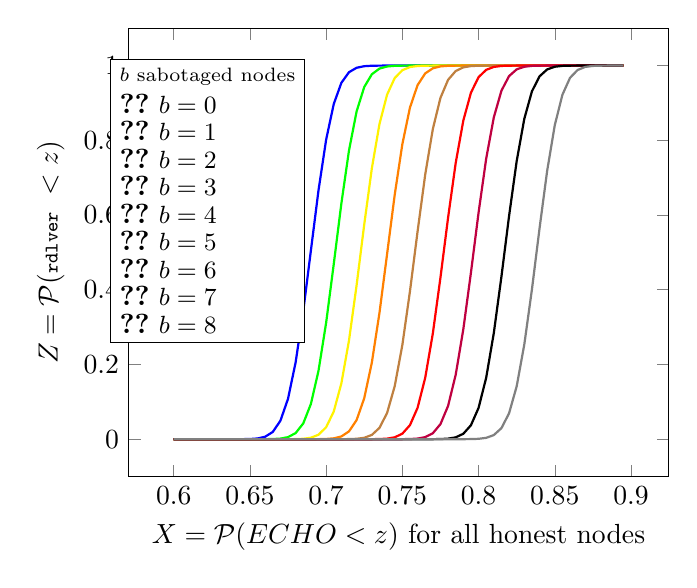
\begin{tikzpicture}
\begin{axis}[ 
    xlabel={$X = \mathcal{P}(ECHO < z)$ for all honest nodes},
    ylabel={$Z = \mathcal{P}({\scriptstyle\mathtt{rdlver}} ~ < z)$},
    ylabel near ticks,
]
  
\addplot[blue,thick] coordinates {
(0.6,7.381302483201029e-14)(0.605,1.4274422092481772e-12)(0.61,2.3640287899482728e-11)(0.615,3.35061485269394e-10)(0.62,4.061641311391178e-09)(0.625,4.208626703361768e-08)(0.63,3.725956277975355e-07)(0.635,2.817375392430534e-06)(0.64,1.819216568829287e-05)(0.645,0.00010031697704821041)(0.65,0.000472559322382775)(0.655,0.001902981482004006)(0.66,0.006558873825995439)(0.665,0.019384221346348204)(0.67,0.04925907210538647)(0.675,0.10805842114372206)(0.68,0.20577025217545059)(0.685,0.34277194314457987)(0.6900000000000001,0.5047380074491797)(0.6950000000000001,0.6660903979596449)(0.7000000000000001,0.8014634127933268)(0.7050000000000001,0.8970645337147377)(0.7100000000000001,0.9538649754638273)(0.7150000000000001,0.9822437643853553)(0.7200000000000001,0.9941614798069274)(0.7250000000000001,0.9983663805059899)(0.7300000000000001,0.9996122864190198)(0.7350000000000001,0.9999221521059732)(0.7400000000000001,0.9999868055607156)(0.7450000000000001,0.9999981159958161)(0.7500000000000001,0.9999997737892442)(0.7550000000000001,0.9999999772023577)(0.7600000000000001,0.9999999980751855)(0.7650000000000001,0.9999999998641301)(0.7700000000000001,0.9999999999919996)(0.7750000000000001,0.999999999999608)(0.7800000000000001,0.999999999999984)(0.7850000000000001,0.9999999999999996)(0.7900000000000001,0.9999999999999999)(0.7950000000000002,1.0)(0.8000000000000002,1.0)(0.8050000000000002,1.0)(0.8100000000000002,1.0)(0.8150000000000002,1.0)(0.8200000000000002,1.0)(0.8250000000000002,1.0)(0.8300000000000002,1.0)(0.8350000000000002,1.0)(0.8400000000000002,1.0)(0.8450000000000002,1.0)(0.8500000000000002,1.0)(0.8550000000000002,1.0)(0.8600000000000002,1.0)(0.8650000000000002,1.0)(0.8700000000000002,1.0)(0.8750000000000002,1.0)(0.8800000000000002,1.0)(0.8850000000000002,1.0)(0.8900000000000002,1.0)(0.8950000000000002,1.0)
};\label{b0}
\addplot[green,thick] coordinates {
(0.6,4.490759699730653e-18)(0.605,1.3091256482147663e-16)(0.61,3.290755956088118e-15)(0.615,7.127511475451589e-14)(0.62,1.3291666237089564e-12)(0.625,2.1325235805669003e-11)(0.63,2.94146667413955e-10)(0.635,3.4856945936756715e-09)(0.64,3.5464644692661476e-08)(0.645,3.0963145614907244e-07)(0.65,2.3187285343546966e-06)(0.655,1.4889789783934367e-05)(0.66,8.198353662527215e-05)(0.665,0.000387118564055316)(0.67,0.001568449722394253)(0.675,0.005458016675069293)(0.68,0.01633914126212621)(0.685,0.042179364351342286)(0.6900000000000001,0.09422580811501184)(0.6950000000000001,0.1830634404571597)(0.7000000000000001,0.31146488222125285)(0.7050000000000001,0.4684950693341753)(0.7100000000000001,0.6308731067656775)(0.7150000000000001,0.7727492647193246)(0.7200000000000001,0.8774263865080018)(0.7250000000000001,0.9426026580398292)(0.7300000000000001,0.976829559971615)(0.7350000000000001,0.9919803924137852)(0.7400000000000001,0.9976303699655735)(0.7450000000000001,0.9994043216190583)(0.7500000000000001,0.9998729726115105)(0.7550000000000001,0.9999770776533079)(0.7600000000000001,0.9999965075989335)(0.7650000000000001,0.99999955169857)(0.7700000000000001,0.9999999516186366)(0.7750000000000001,0.9999999956198408)(0.7800000000000001,0.9999999996681297)(0.7850000000000001,0.9999999999790126)(0.7900000000000001,0.9999999999988956)(0.7950000000000002,0.9999999999999518)(0.8000000000000002,0.9999999999999982)(0.8050000000000002,1.0)(0.8100000000000002,1.0)(0.8150000000000002,1.0)(0.8200000000000002,1.0)(0.8250000000000002,1.0)(0.8300000000000002,1.0)(0.8350000000000002,1.0)(0.8400000000000002,1.0)(0.8450000000000002,1.0)(0.8500000000000002,1.0)(0.8550000000000002,1.0)(0.8600000000000002,1.0)(0.8650000000000002,1.0)(0.8700000000000002,1.0)(0.8750000000000002,1.0)(0.8800000000000002,1.0)(0.8850000000000002,1.0)(0.8900000000000002,1.0)(0.8950000000000002,1.0)
};\label{b1}
\addplot[yellow,thick] coordinates {
(0.6,5.552137285219799e-23)(0.605,2.4142287054306263e-21)(0.61,9.114704900562854e-20)(0.615,2.9856993595941135e-18)(0.62,8.479363913991896e-17)(0.625,2.086190770918722e-15)(0.63,4.442914488445941e-14)(0.635,8.183696485892055e-13)(0.64,1.3026970678664695e-11)(0.645,1.7906098477952826e-10)(0.65,2.123669760957271e-09)(0.655,2.171642123200288e-08)(0.66,1.9134773676931015e-07)(0.665,1.4519593771410716e-06)(0.67,9.484239018891177e-06)(0.675,5.3316984276801864e-05)(0.68,0.00025795474251028976)(0.685,0.0010744090390422674)(0.6900000000000001,0.003855259085448833)(0.6950000000000001,0.011932704018399812)(0.7000000000000001,0.03192140293584917)(0.7050000000000001,0.07402178338990954)(0.7100000000000001,0.14942155213264618)(0.7150000000000001,0.2641426852825466)(0.7200000000000001,0.4123019911599361)(0.7250000000000001,0.5745819231262596)(0.7300000000000001,0.725209411120839)(0.7350000000000001,0.8435990672391458)(0.7400000000000001,0.9223346522463106)(0.7450000000000001,0.9666099537785198)(0.7500000000000001,0.9876464649445758)(0.7550000000000001,0.9960855104373783)(0.7600000000000001,0.998941756361155)(0.7650000000000001,0.9997567154107597)(0.7700000000000001,0.9999525717389982)(0.7750000000000001,0.9999921794128486)(0.7800000000000001,0.9999989119290262)(0.7850000000000001,0.9999998725837225)(0.7900000000000001,0.9999999874735761)(0.7950000000000002,0.9999999989690105)(0.8000000000000002,0.9999999999291795)(0.8050000000000002,0.9999999999959541)(0.8100000000000002,0.9999999999998085)(0.8150000000000002,0.9999999999999926)(0.8200000000000002,0.9999999999999998)(0.8250000000000002,1.0)(0.8300000000000002,1.0)(0.8350000000000002,1.0)(0.8400000000000002,1.0)(0.8450000000000002,1.0)(0.8500000000000002,1.0)(0.8550000000000002,1.0)(0.8600000000000002,1.0)(0.8650000000000002,1.0)(0.8700000000000002,1.0)(0.8750000000000002,1.0)(0.8800000000000002,1.0)(0.8850000000000002,1.0)(0.8900000000000002,1.0)(0.8950000000000002,1.0)
};\label{b2}
\addplot[orange,thick] coordinates {
(0.6,1.2600681673183202e-28)(0.605,8.092674399417694e-27)(0.61,4.542844238927972e-25)(0.615,2.2276597172455598e-23)(0.62,9.53616281790405e-22)(0.625,3.5611867248720274e-20)(0.63,1.1592619308378981e-18)(0.635,3.2868805931946146e-17)(0.64,8.110274941565199e-16)(0.645,1.7400362768901744e-14)(0.65,3.243144686129219e-13)(0.655,5.2465189957934125e-12)(0.66,7.360166712694598e-11)(0.665,8.946217448789781e-10)(0.67,9.413851384826357e-09)(0.675,8.569146678547573e-08)(0.68,6.742991649540132e-07)(0.685,4.584206930813354e-06)(0.6900000000000001,2.69147179400982e-05)(0.6950000000000001,0.0001364375129154867)(0.7000000000000001,0.0005971930898105093)(0.7050000000000001,0.002257887708400277)(0.7100000000000001,0.007380165234521924)(0.7150000000000001,0.02088537946752232)(0.7200000000000001,0.05128912497640915)(0.7250000000000001,0.10967053910229733)(0.7300000000000001,0.20519004223285373)(0.7350000000000001,0.3382174785157614)(0.7400000000000001,0.4957599443108437)(0.7450000000000001,0.6542674663075086)(0.7500000000000001,0.7896298809584531)(0.7550000000000001,0.8876582200038442)(0.7600000000000001,0.9478068269158265)(0.7650000000000001,0.9790486059615017)(0.7700000000000001,0.9927729777256048)(0.7750000000000001,0.9978673671130456)(0.7800000000000001,0.9994636391599604)(0.7850000000000001,0.9998854055000215)(0.7900000000000001,0.9999792631746713)(0.7950000000000002,0.9999968307662706)(0.8000000000000002,0.9999995920965056)(0.8050000000000002,0.9999999559190506)(0.8100000000000002,0.9999999960132054)(0.8150000000000002,0.9999999996993202)(0.8200000000000002,0.9999999999811676)(0.8250000000000002,0.999999999999025)(0.8300000000000002,0.9999999999999585)(0.8350000000000002,0.9999999999999986)(0.8400000000000002,1.0)(0.8450000000000002,1.0)(0.8500000000000002,1.0)(0.8550000000000002,1.0)(0.8600000000000002,1.0)(0.8650000000000002,1.0)(0.8700000000000002,1.0)(0.8750000000000002,1.0)(0.8800000000000002,1.0)(0.8850000000000002,1.0)(0.8900000000000002,1.0)(0.8950000000000002,1.0)
};\label{b3}
\addplot[brown,thick] coordinates {
(0.6,4.6338558836798983e-35)(0.605,4.358344290099576e-33)(0.61,3.605393348094237e-31)(0.615,2.622171202541739e-29)(0.62,1.6758569421817385e-27)(0.625,9.40670151109613e-26)(0.63,4.63434132659664e-24)(0.635,2.002559658598713e-22)(0.64,7.584020353509232e-21)(0.645,2.515218634057736e-19)(0.65,7.298583973501351e-18)(0.655,1.8513750506827398e-16)(0.66,4.101426020109614e-15)(0.665,7.927588601115528e-14)(0.67,1.3356350594904957e-12)(0.675,1.9595137394994775e-11)(0.68,2.500921800382606e-10)(0.685,2.774159370356237e-09)(0.6900000000000001,2.6720757887119606e-08)(0.6950000000000001,2.2329879351560246e-07)(0.7000000000000001,1.6177717718042696e-06)(0.7050000000000001,1.015470566395389e-05)(0.7100000000000001,5.5199266396250875e-05)(0.7150000000000001,0.0002597799304737998)(0.7200000000000001,0.0010585191608465697)(0.7250000000000001,0.0037358694679684155)(0.7300000000000001,0.01143095694467093)(0.7350000000000001,0.030371262081300525)(0.7400000000000001,0.07024546828375229)(0.7450000000000001,0.14195983583024036)(0.7500000000000001,0.2520169347368248)(0.7550000000000001,0.3959723032857317)(0.7600000000000001,0.5562771311502266)(0.7650000000000001,0.7080851713304951)(0.7700000000000001,0.830208885440989)(0.7750000000000001,0.913575746326897)(0.7800000000000001,0.9618154617789166)(0.7850000000000001,0.9854504371736527)(0.7900000000000001,0.9952441811503203)(0.7950000000000002,0.9986723405461024)(0.8000000000000002,0.9996846767502672)(0.8050000000000002,0.9999365099220731)(0.8100000000000002,0.9999891986423121)(0.8150000000000002,0.9999984525580667)(0.8200000000000002,0.9999998139672635)(0.8250000000000002,0.9999999813038545)(0.8300000000000002,0.9999999984359038)(0.8350000000000002,0.9999999998915987)(0.8400000000000002,0.9999999999938103)(0.8450000000000002,0.9999999999997107)(0.8500000000000002,0.999999999999989)(0.8550000000000002,0.9999999999999997)(0.8600000000000002,1.0)(0.8650000000000002,1.0)(0.8700000000000002,1.0)(0.8750000000000002,1.0)(0.8800000000000002,1.0)(0.8850000000000002,1.0)(0.8900000000000002,1.0)(0.8950000000000002,1.0)
};\label{b4}
\addplot[red,thick] coordinates {
(0.6,2.364813344955456e-42)(0.605,3.2354810817713358e-40)(0.61,3.9158560140041537e-38)(0.615,4.191555174130789e-36)(0.62,3.966995860449795e-34)(0.625,3.318389078959961e-32)(0.63,2.4523200723127377e-30)(0.635,1.6002288005546525e-28)(0.64,9.214668236498675e-27)(0.645,4.679246848859037e-25)(0.65,2.0938561132398896e-23)(0.655,8.249741080898141e-22)(0.66,2.859423897502257e-20)(0.665,8.710843239329869e-19)(0.67,2.330039094347256e-17)(0.675,5.466982636799067e-16)(0.68,1.1239818457442582e-14)(0.685,2.0227065769368072e-13)(0.6900000000000001,3.182707877959968e-12)(0.6950000000000001,4.3739875609292865e-11)(0.7000000000000001,5.244517948418252e-10)(0.7050000000000001,5.480518432218701e-09)(0.7100000000000001,4.986372133611383e-08)(0.7150000000000001,3.9462200379523845e-07)(0.7200000000000001,2.714172192680213e-06)(0.7250000000000001,1.6211862849433018e-05)(0.7300000000000001,8.404668543624342e-05)(0.7350000000000001,0.0003780509357421106)(0.7400000000000001,0.0014753716898343232)(0.7450000000000001,0.004997190946078145)(0.7500000000000001,0.014703031545204508)(0.7550000000000001,0.03763900516953668)(0.7600000000000001,0.08404903105137418)(0.7650000000000001,0.1643494583245149)(0.7700000000000001,0.28299312315754815)(0.7750000000000001,0.4324821079609985)(0.7800000000000001,0.5928937607808099)(0.7850000000000001,0.7392979319826781)(0.7900000000000001,0.8527968095084676)(0.7950000000000002,0.9274375400167191)(0.8000000000000002,0.9690210109143693)(0.8050000000000002,0.9886193699446855)(0.8100000000000002,0.9964218619571192)(0.8150000000000002,0.9990416945091547)(0.8200000000000002,0.9997822954887845)(0.8250000000000002,0.9999582165724659)(0.8300000000000002,0.999993251919642)(0.8350000000000002,0.9999990867418801)(0.8400000000000002,0.9999998968907603)(0.8450000000000002,0.9999999903366661)(0.8500000000000002,0.9999999992524854)(0.8550000000000002,0.999999999952583)(0.8600000000000002,0.9999999999975522)(0.8650000000000002,0.9999999999998981)(0.8700000000000002,0.9999999999999966)(0.8750000000000002,0.9999999999999999)(0.8800000000000002,1.0)(0.8850000000000002,1.0)(0.8900000000000002,1.0)(0.8950000000000002,1.0)
};\label{b5}
\addplot[purple,thick] coordinates {
(0.6,1.3794819724785658e-50)(0.605,2.732755287269643e-48)(0.61,4.813876484817752e-46)(0.615,7.540572447924174e-44)(0.62,1.0502626744389768e-41)(0.625,1.300493701388376e-39)(0.63,1.431302057303474e-37)(0.635,1.3996739982101e-35)(0.64,1.215679609726593e-33)(0.645,9.373394825882219e-32)(0.65,6.412312665453991e-30)(0.655,3.8894966272550527e-28)(0.66,2.0903620754331808e-26)(0.665,9.946180829434914e-25)(0.67,4.186253229835482e-23)(0.675,1.5571430545614268e-21)(0.68,5.113742099543109e-20)(0.685,1.4811731540399797e-18)(0.6900000000000001,3.77970015728131e-17)(0.6950000000000001,8.487939519557178e-16)(0.7000000000000001,1.6754585155641142e-14)(0.7050000000000001,2.903569739633316e-13)(0.7100000000000001,4.412354112964972e-12)(0.7150000000000001,5.872412596202124e-11)(0.7200000000000001,6.836615062258031e-10)(0.7250000000000001,6.953803595548426e-09)(0.7300000000000001,6.172408446833631e-08)(0.7350000000000001,4.775923837988672e-07)(0.7400000000000001,3.21800941903878e-06)(0.7450000000000001,1.886484015779148e-05)(0.7500000000000001,9.614678143200101e-05)(0.7550000000000001,0.00042580255719178314)(0.7600000000000001,0.0016382459556118884)(0.7650000000000001,0.0054767960518507216)(0.7700000000000001,0.015920777758650115)(0.7750000000000001,0.040301639466228015)(0.7800000000000001,0.08905568889039296)(0.7850000000000001,0.1724333909607434)(0.7900000000000001,0.29418361806992555)(0.7950000000000002,0.44574079805946276)(0.8000000000000002,0.6063156547440423)(0.8050000000000002,0.7508856001520803)(0.8100000000000002,0.8613126981004519)(0.8150000000000002,0.9327546655076923)(0.8200000000000002,0.9718360002716315)(0.8250000000000002,0.9898804508243623)(0.8300000000000002,0.996898898363427)(0.8350000000000002,0.9991937225024371)(0.8400000000000002,0.9998230147698969)(0.8450000000000002,0.9999673579023718)(0.8500000000000002,0.999994966769039)(0.8550000000000002,0.9999993546104902)(0.8600000000000002,0.9999999315891325)(0.8650000000000002,0.9999999940458257)(0.8700000000000002,0.9999999995778066)(0.8750000000000002,0.9999999999758337)(0.8800000000000002,0.9999999999988953)(0.8850000000000002,0.9999999999999603)(0.8900000000000002,0.9999999999999989)(0.8950000000000002,1.0)
};\label{b6}
\addplot[black,thick] coordinates {
(0.6,7.20639433579172e-60)(0.605,2.0617728825448762e-57)(0.61,5.270222784320385e-55)(0.615,1.2038488838721328e-52)(0.62,2.457681001858419e-50)(0.625,4.484469320985335e-48)(0.63,7.313335531523915e-46)(0.635,1.0658371412005942e-43)(0.64,1.3878867300314968e-41)(0.645,1.6143091227032923e-39)(0.65,1.6766225513804116e-37)(0.655,1.5542149143805972e-35)(0.66,1.2852578891784884e-33)(0.665,9.475771132932323e-32)(0.67,6.22431295622679e-30)(0.675,3.639945142789216e-28)(0.68,1.893503404648175e-26)(0.685,8.754164561200148e-25)(0.6900000000000001,3.593516316284322e-23)(0.6950000000000001,1.3083698240359672e-21)(0.7000000000000001,4.22055330943342e-20)(0.7050000000000001,1.2048481673215214e-18)(0.7100000000000001,3.040125782340529e-17)(0.7150000000000001,6.771701957310517e-16)(0.7200000000000001,1.3297902627044644e-14)(0.7250000000000001,2.2991316420356573e-13)(0.7300000000000001,3.4949766320999236e-12)(0.7350000000000001,4.6646724810673665e-11)(0.7400000000000001,5.458692100879329e-10)(0.7450000000000001,5.5929930633739474e-09)(0.7500000000000001,5.0106826508018595e-08)(0.7550000000000001,3.919903416333121e-07)(0.7600000000000001,2.674486111492198e-06)(0.7650000000000001,1.5896403737866745e-05)(0.7700000000000001,8.222867670336049e-05)(0.7750000000000001,0.00036989285939381965)(0.7800000000000001,0.0014462457784042062)(0.7850000000000001,0.004914443023391035)(0.7900000000000001,0.014519533990693737)(0.7950000000000002,0.03733942646638733)(0.8000000000000002,0.08375932145574609)(0.8050000000000002,0.16445227221139452)(0.8100000000000002,0.2840899949654839)(0.8150000000000002,0.43508342349956913)(0.8200000000000002,0.5969862674381633)(0.8250000000000002,0.744181729766091)(0.8300000000000002,0.8574205302696031)(0.8350000000000002,0.9309809648025769)(0.8400000000000002,0.9712419549855555)(0.8450000000000002,0.9897642784020144)(0.8500000000000002,0.996908734986278)(0.8550000000000002,0.9992127129306557)(0.8600000000000002,0.9998319211071699)(0.8650000000000002,0.999970102712215)(0.8700000000000002,0.9999955978033974)(0.8750000000000002,0.9999994672734657)(0.8800000000000002,0.9999999474494117)(0.8850000000000002,0.9999999958145223)(0.8900000000000002,0.99999999973386)(0.8950000000000002,0.99999999998667)
};\label{b7}
\addplot[gray,thick] coordinates {
(0.6,2.4756872141075086e-70)(0.605,1.022319037299543e-67)(0.61,3.7882407147086e-65)(0.615,1.260115732260547e-62)(0.62,3.763884919435818e-60)(0.625,1.009755004073241e-57)(0.63,2.4334313597158446e-55)(0.635,5.26845854759777e-53)(0.64,1.0247435029981478e-50)(0.645,1.7905519822376544e-48)(0.65,2.810208986271831e-46)(0.655,3.960739650275632e-44)(0.66,5.011548456969303e-42)(0.665,5.690665557560452e-40)(0.67,5.796322256046035e-38)(0.675,5.293078069645131e-36)(0.68,4.330753447382818e-34)(0.685,3.1726064101915956e-32)(0.6900000000000001,2.079361510949317e-30)(0.6950000000000001,1.2182430702630912e-28)(0.7000000000000001,6.374162783845554e-27)(0.7050000000000001,2.97549568103269e-25)(0.7100000000000001,1.2378600813980632e-23)(0.7150000000000001,4.584133248015254e-22)(0.7200000000000001,1.509326339643338e-20)(0.7250000000000001,4.412522001423039e-19)(0.7300000000000001,1.1438744814765155e-17)(0.7350000000000001,2.6256801235393235e-16)(0.7400000000000001,5.328904319225722e-15)(0.7450000000000001,9.547871111610471e-14)(0.7500000000000001,1.5078907120110193e-12)(0.7550000000000001,2.09573398312582e-11)(0.7600000000000001,2.559200879233725e-10)(0.7650000000000001,2.7413832363407236e-09)(0.7700000000000001,2.5717612959955874e-08)(0.7750000000000001,2.109585748388656e-07)(0.7800000000000001,1.5107826369212378e-06)(0.7850000000000001,9.432224343676583e-06)(0.7900000000000001,5.126925714852237e-05)(0.7950000000000002,0.00024234391820149876)(0.8000000000000002,0.0009952916693889923)(0.8050000000000002,0.0035495623808005188)(0.8100000000000002,0.010992054076624609)(0.8150000000000002,0.029575118044370397)(0.8200000000000002,0.06924414999588847)(0.8250000000000002,0.14147093676263814)(0.8300000000000002,0.25336896078002924)(0.8350000000000002,0.40052363890221965)(0.8400000000000002,0.5643876661182253)(0.8450000000000002,0.7185059841695653)(0.8500000000000002,0.8406159620134109)(0.8550000000000002,0.9218964309848724)(0.8600000000000002,0.9672171915630554)(0.8650000000000002,0.988319009895169)(0.8700000000000002,0.9964952061758036)(0.8750000000000002,0.9991212516140198)(0.8800000000000002,0.9998172950017339)(0.8850000000000002,0.999968753315039)(0.8900000000000002,0.9999956433721038)(0.8950000000000002,0.9999995098079202)
};\label{b8}

\end{axis}
\node [draw,fill=white] at (1,3.5) {\shortstack[l]{
{\scriptsize $b$ sabotaged nodes}\\
\ref{b0} {\small $b = 0$}\\
\ref{b1} {\small $b = 1$}\\
\ref{b2} {\small $b = 2$}\\
\ref{b3} {\small $b = 3$}\\
\ref{b4} {\small $b = 4$}\\
\ref{b5} {\small $b = 5$}\\
\ref{b6} {\small $b = 6$}\\
\ref{b7} {\small $b = 7$}\\
\ref{b8} {\small $b = 8$}
}
};
\end{tikzpicture}
}

    \caption{Theoretical effect of Bracha sabotage for $n=25$}
    \label{fig:bracha_sabotage_theory}
\vspace*{-.25cm}
\end{figure}


Via plotting this probability $Z$ w.r.t.~$X$ on Fig.\ref{fig:bracha_sabotage_theory} (with $n=25$ and $f=8$), we observe that the more nodes are sabotaged, the less likely is the occurrence of the delivery $\mathtt{rdlver}$ operation before timestamp $z$.
Consequently, even if we stay below the maximum number $f$ of Byzantine nodes, sabotage can still result in the delivery of vertices to be delayed (statistically).
In turn, if the delivery of vertices that contain transactions from the target client is delayed, this makes them less likely to be the target of strong edges (which may result in situations such as the one described in Sec.\ref{ssec:attack_bracha} and Fig.\ref{fig:dag_attacked_bracha_layer}).
This can be partly mitigated by DagRider supporting weak edges.
The mitigation is only partial because for the delayed vertex to be included in the next wave $w$, it still requires to be targeted (via a weak edge) by a vertex in the causal subgraph of $w$'s leader. Otherwise it won't be included until at least wave $w+1$.



\section{Details of the 10 DAG-specific OF properties\label{anx:enumeration_order_fairness_props}}

The 8 properties, covering all $OF^\beta_\alpha$ cases of Sec.\ref{ssec:metrics} are:\\
\noindent$\bullet$ $OF^{F_{IN}}_{S_{ND}}$ as ``finalization-order-fairness w.r.t.~transaction emission'': if the initial emission of $x$ by a certain client precedes that of $x'$ then all honest nodes must finalize $x$ before $x'$.\\
\noindent$\bullet$ $OF^{W_{AV}}_{S_{ND}}$ as ``wave-order-fairness w.r.t.~transaction emission'': if the initial emission of $x$ by a certain client precedes that of $x'$ then no honest node can finalize $x'$ in a wave before that in which $x$ is finalized.\\
\noindent$\bullet$ $OF^{F_{IN}}_{R_{EC}}$ as ``finalization-order-fairness w.r.t.~reception from client'': if a majority of nodes receive $x$ from a client before they do so for $x'$ then all honest nodes must finalize $x$ before $x'$.\\
\noindent$\bullet$ $OF^{W_{AV}}_{R_{EC}}$ as ``wave-order-fairness w.r.t.~reception from client'': if a majority of nodes receive $x$ from a client before they do so for $x'$ then no honest node can finalize $x'$ in a wave before that in which $x$ is finalized.\\
\noindent$\bullet$ $OF^{F_{IN}}_{I_{NI}}$ as ``finalization-order-fairness w.r.t.~broadcast initiation'': if a majority of nodes begin their participation in the reliable broadcast of a vertex that contains $x$ before they do so for $x'$ then all honest nodes must finalize $x$ before $x'$.\\
\noindent$\bullet$ $OF^{W_{AV}}_{I_{NI}}$ as ``wave-order-fairness w.r.t.~broadcast initiation'': if a majority of nodes begin their participation in the reliable broadcast of a vertex that contains $x$ before they do so for $x'$ then no honest node can finalize $x'$ in a wave before that in which $x$ is finalized.\\
\noindent$\bullet$ $OF^{F_{IN}}_{D_{LV}}$ as ``finalization-order-fairness w.r.t.~broadcast delivery'': if a majority of nodes deliver a vertex containing $x$ before they do so for $x'$ then all honest nodes must finalize $x$ before $x'$.\\
\noindent$\bullet$ $OF^{W_{AV}}_{D_{LV}}$ as ``wave-order-fairness w.r.t.~broadcast delivery'': if a majority of nodes deliver a vertex containing $x$ before they do so for $x'$ then no honest node can finalize $x'$ in a wave before that in which $x$ is finalized.



\section{Details on simulation parameterization\label{anx:max_sim}}


We use the MAX Multi-Agent eXperimenter tool \cite{max_tool}, which is based on the Agent-Group-Role \cite{from_agents_to_organizations_an_organizational_view_of_multi_agent_systems} Multi-Agent System \cite{an_introduction_to_multiagent_systems} formalism.
It allows discrete time simulation of complex distributed systems.
Our implementation of DagRider \cite{all_you_need_is_dag} is available in \cite{max_dagrider} and that of the underlying Bracha BRB algorithm \cite{on_the_versatility_of_bracha_byzantine_reliable_broadcast_algorithm} in \cite{max_bracha}.
We use the adversary model defined in \cite{adversary_augmented_simulation_to_evaluate_client_fairness_on_hyperledger_fabric} and implemented in \cite{max_p2p_adversarial_model}. 

Fig.\ref{fig:network_param} describes the parameterization of the system, with the colors of the delay distributions corresponding to the curves on Fig.\ref{fig:delays_distros} (except from the constant rate \textcolor{orange}{\faDashboard} at which new puzzles are revealed).


\begin{figure}[h]
\vspace*{-.25cm}
    \centering
    \scalebox{1}{\begin{tikzpicture}
%
%
% === ENTITIES
%
\node[draw,diamond] at (0,1) (client1) {$\chi_1$};
\node at (-.25,0) {\rotatebox{90}{\Large$\cdots$}};
\node[draw,diamond,inner sep=1.75] at (0,-1) (clientm) {$\chi_{m}$};
%
\node[draw,circle] at (1.75,1.25) (n1) {$\eta_1$};
\node[draw,circle] at (1.75,.5) (n2) {$\eta_2$};
\node at (1.75,-.25) {\rotatebox{90}{\Large$\cdots$}};
\node[draw,circle] at (1.75,-1.25) (nn) {$\eta_n$};
%
\node[draw,rectangle] at (-1,0) (puzzler) {\textcolor{orange}{\faDashboard}};
%
%
%
% === ARROWS
%
\draw (puzzler) edge[->,bend left=5] node[pos=.6,circle,fill=white,inner sep=-.5] {\textcolor{yellow}{\faLightbulbO}} (client1);
\draw (puzzler) edge[->,bend right=5] node[pos=.6,circle,fill=white,inner sep=-.5] {\textcolor{yellow}{\faLightbulbO}} (clientm);
%
\node[align=center] at (-1.1,-.7) {\scriptsize puzzles};
%
%
\draw (client1) edge[->,bend left=20] node[pos=.25,circle,fill=white,inner sep=-.5] {\scriptsize\textcolor{red}{\faHourglassO}} (n1);
\draw (client1) edge[->,bend left=5] node[pos=.25,circle,fill=white,inner sep=-.5] {\scriptsize\textcolor{red}{\faHourglassO}} (n2);
\draw (client1) edge[->,bend right=20] node[pos=.1,circle,fill=white,inner sep=-.5] {\scriptsize\textcolor{red}{\faHourglassO}} (nn);
%
\draw (clientm) edge[->,bend left=20] node[pos=.1,circle,fill=white,inner sep=-.5] {\scriptsize\textcolor{red}{\faHourglassO}} (n1);
\draw (clientm) edge[->,bend right=5] node[pos=.1,circle,fill=white,inner sep=-.5] {\scriptsize\textcolor{red}{\faHourglassO}} (n2);
\draw (clientm) edge[->,bend right=5] node[pos=.25,circle,fill=white,inner sep=-.5] {\scriptsize\textcolor{red}{\faHourglassO}} (nn);
%
\node[align=center] at (.8,-1.6) {\scriptsize transactions};
%
%
\draw (n1.350) edge[<->,bend left=45] node[midway,circle,fill=white,inner sep=-.5] {\textcolor{black}{\faClockO}} (n2.10);
%
\draw (n2.350) edge[<->,bend left=55] node[midway,circle,fill=white,inner sep=-.5] {\textcolor{black}{\faClockO}} (nn.10);
%
\draw (nn.350) edge[<->,bend right=65] node[midway,circle,fill=white,inner sep=-.5] {\textcolor{black}{\faClockO}} (n1.10);
%
\node[align=center] at (2.7,-1.35) {\scriptsize Bracha};
\node[align=center] at (2.7,-1.65) {\scriptsize messages};
%
%
% === LEGEND
%
\node[draw,line width=1.25,inner sep=2] at (5,0.25) {
\begin{tikzpicture}
\node (leg1) at (0,0) {$\chi$ {\scriptsize Clients ($m$ in total)}};
\node[below=0.15cm of leg1.south west, anchor=north west] (leg2) {$\eta$ {\scriptsize Nodes ($n$ in total)}};
\node[below=0.15cm of leg2.south west, anchor=north west] (leg3) {Delay distributions:};
\node[below=0.1cm of leg3.south west, anchor=north west] (leg4) {\textcolor{orange}{\faDashboard} {\scriptsize Constant} ~~ \textcolor{yellow}{\faLightbulbO} {\scriptsize Poisson}};
\node[below=0.1cm of leg4.south west, anchor=north west] (leg5) {\textcolor{red}{\faHourglassO} {\scriptsize Exponential}};
\node[below=0.1cm of leg5.south west, anchor=north west] (leg6) {\textcolor{blue}{\faClockO}/\textcolor{green}{\faClockO} {\scriptsize Hypoexponential}};
\end{tikzpicture}
};
\end{tikzpicture}}
    \caption{Network parameterization}
    \label{fig:network_param}
\vspace*{-.25cm}
\end{figure}


We use an arbitrary unit of time denoted as ``tick'' in our discrete time simulations.
We consider that a new puzzle is revealed every 200 ticks \textcolor{orange}{\faDashboard}.
Any client can solve it after a given time that is modeled by a Poisson distribution \textcolor{yellow}{\faLightbulbO} of mean 100 (in ticks).
Once a client solves a puzzle, it creates a transaction and broadcasts it to nodes.
We consider the \textcolor{red}{\faHourglassO} distribution of delays taken by such transactions to reach any given node to be an Exponential distribution of mean 20.

As for the delay \textcolor{black}{\faClockO} of node to node communications, we consider 2 different cases in order to model quicker and slower P2P networks:
\begin{itemize}
    \item a hypoexponential distribution \textcolor{blue}{\faClockO} with rates (1/10, 1/15 and 1/20) modelling an average P2P network with smaller delays
    \item a hypoexponential distribution \textcolor{green}{\faClockO} with rates (1/20, 1/30 and 1/40) modelling a slow P2P network with larger delays
\end{itemize}


\begin{figure}[h]
\vspace*{-.25cm}
    \centering
    \includegraphics[width=.475\textwidth]{images/delays_distros_rw.png}
    \caption{Distributions of delays (log scale)}
    \label{fig:delays_distros}
\vspace*{-.25cm}
\end{figure}





\section{Details on simulation execution\label{anx:max_sim_exec}}


Running a simulation yields client puzzle solutions being included in the local copies of the DAG hosted on each node.
In the following, we consider a simple case with $3$ clients and $4$ nodes which are all honest.
The diagrams on Fig.\ref{fig:dag_simu_further_discussion} and Fig.\ref{fig:dag_from_simu} are produced by our tool. 
Each corresponds to a representation of the local copy of the DAG at a certain node at the end of the simulation. 
Here, strong edges are drawn in red and weak edges in blue.
Vertices framed in red are leaders.
The colors of the vertices correspond to the wave they are finalized in (white vertices are not yet included in any wave).


\begin{figure}[h]
    \centering

    \begin{subfigure}{.475\textwidth}
        \includegraphics[scale=.28]{images/simu_baseline_perfect_network.png}
        \caption{simulation with a perfect network}
        \label{fig:dag_from_simu_perfect}
    \end{subfigure}
    
    \begin{subfigure}{.475\textwidth}
        \includegraphics[scale=.28]{images/SmallDelays_0byznode_cropped2.png}
        \caption{simulation to illustrate leader skipping}
        \label{fig:dag_from_simu_quickest}
    \end{subfigure}
    
    \caption{Simulation examples}
    \label{fig:dag_simu_further_discussion}
\end{figure}


Fig.\ref{fig:dag_from_simu_perfect} results from a simulation in which there are no third party transactions and in which both \textcolor{red}{\faHourglassO} and \textcolor{black}{\faClockO} are s.t.~there is always the same fixed delay of $1$ simulation tick between the moment an emission or reception is scheduled and executed in the reliable broadcast layer and there is always a delay of $1$ between the moment a new puzzle is revealed and the moment a node receives its solution from its corresponding client.
This allows every node to produce a new vertex as soon as it receives the solutions (which all arrive at the same time) from the clients at exactly the rate in which puzzles are revealed.
Here, it is as if the construction of the DAG is executed in lock-step synchrony across all nodes.
As a result, every vertex has exactly $n = 4$ strong edges and no weak edge.
In these conditions, the adversary cannot delay the delivery of vertices i.e., the attack on the reliable broadcast layer from Sec.\ref{ssec:attack_bracha} has no effect.
The DagRider layer attack from Sec.\ref{ssec:byz_dagrider_layer} is also ineffective because, even if a Byzantine node at column $c$ decides not to include strong edges to certain vertices at column $c-1$, it must include $2*f+1$ strong edges and at least $f+1$ of these targeted vertices will, in any case, include all the pending puzzle solutions.
Here, the adversary can only manipulate the content of the DAG via Byzantine nodes not including certain transactions in their own vertices proposal.

In contrast, on Fig.\ref{fig:dag_from_simu_quickest}, we use a hypoexponential distribution of delays for node to node communications. One can see that the regularity of the DAG is broken : weak edges appear and the shape of the waves vary.

%Communication models \cite{consensus_in_the_presence_of_partial_synchrony,impossibility_of_distributed_consensus_with_one_faulty_process} describe assumptions on the communication delays under which the properties of a distributed protocol hold.
This comparison with a perfect network shows that it is the non-determinism in network communication delays that leave Byzantine nodes with ample leeway to change the outcome of an execution via manipulating these delays.
This is true, even when staying within the $\Delta$ bounds in a synchronous or partially synchronous communication model \cite{consensus_in_the_presence_of_partial_synchrony,impossibility_of_distributed_consensus_with_one_faulty_process}.


The reader may notice that the situation described on Fig.\ref{fig:dagrider_bug} in appendix \ref{anx:bug_dagrider} effectively occurs on Fig.\ref{fig:dag_from_simu_quickest} as it is possible for a vertex at column $c$ and row $r$ to be broadcast ($\mathtt{rbcast}$ of Fig.\ref{fig:layers_dagrider}) before the vertex at column $c-1$ and row $r$ is delivered ($\mathtt{rdlver}$ of Fig.\ref{fig:layers_dagrider}) due to the random delays in the reliable broadcast layer. As a result, there is no strong edge between $(c,r)$ and $(c-1,r)$ (see e.g., the absence of edge between the leader vertex of the orange wave and its immediate predecessor on the same row, which is colored in purple).

Fig.\ref{fig:dag_from_simu_quickest} also illustrates the fact that certain leader vertices can be skipped over.
Indeed, given a leader at column $c$, if the condition that there are at least $2*f+1$ strong paths between it and vertices at column $c + 4$ is not met, it is not included in the leader stack.
In that case, the wave is ignored, and its content may eventually be included in the next wave.
On Fig.\ref{fig:dag_from_simu_quickest}, wave 3 is ignored and its content is included in wave 4 (the orange wave).



In Sec.\ref{ssec:network_param}, we use two specific \faClockO~distributions of delays for our experiments.
Fig.\ref{fig:dag_from_simu} illustrate the use of these two specific distributions.
Fig.\ref{fig:dag_from_simu_quick} results from a simulation with the node to node delay being modeled using the \textcolor{blue}{\faClockO} distribution (smaller delays).
One can see that there are roughly 2 to 3 puzzles per wave of the DAG and 5 to 10 transactions per vertex of the DAG.
On Fig.\ref{fig:dag_from_simu_slow} there rather are roughly 5 to 6 puzzles per wave and 10 to 20 transactions per vertex.


\begin{figure*}
    \centering

\begin{minipage}{.65\textwidth}
    
    \begin{subfigure}{\textwidth}
        \includegraphics[scale=.27]{images/MediumDelays_0byznode_pt.png}
        \caption{...the \textcolor{blue}{\faClockO} (quicker network)}
        \label{fig:dag_from_simu_quick}
    \end{subfigure}
    
\end{minipage}
%
\begin{minipage}{.325\textwidth}
    \begin{subfigure}{\textwidth}
        \includegraphics[scale=.27]{images/LargeDelays_0byznode_pt.png}
        \caption{...the \textcolor{green}{\faClockO} (slower network)}
        \label{fig:dag_from_simu_slow}
    \end{subfigure}
\end{minipage}
    
    \caption{DAG content excerpts at the end of a $n=4$ simulation with ...}
    \label{fig:dag_from_simu}
\end{figure*}





\clearpage 

\section{Additional metrics on the first experiments\label{anx:exp1}}




\begin{figure}[h]
    \centering

\setlength\tabcolsep{1.5pt}
\begin{tabular}{|c|c|}
\hline
{\scriptsize $\#$ of solved puzzles}
&
{\scriptsize $\#$ of waves}
\\
\hline 
\includegraphics[scale=.3]{plots/exp1/exp1_num_solved_puzzles_plot.png}
&
\includegraphics[scale=.3]{plots/exp1/exp1_num_waves_plot.png}
\\
\hline 
\hline
{\scriptsize $\#$ of transactions per wave}
&
{\scriptsize$\#$ of $OF_{I_{NI}}^{W_{AV}}$ violations}
\\
\hline 
\includegraphics[scale=.3]{plots/exp1/exp1_block_size_plot.png}
&
\includegraphics[scale=.3]{plots/exp1/exp1_wavord_wrt_binit_plot.png}
\\
\hline 
\hline
{\scriptsize$\#$ of $OF_{R_{EC}}^{F_{IN}}$ violations}
&
{\scriptsize$\#$ of $OF_{I_{NI}}^{F_{IN}}$ violations}
\\
\hline 
\includegraphics[scale=.3]{plots/exp1/exp1_finord_wrt_rec_plot.png}
&
\includegraphics[scale=.3]{plots/exp1/exp1_finord_wrt_binit_plot.png}
\\
\hline 
\hline 
{\scriptsize$\#$ of $OF_{D_{LV}}^{F_{IN}}$ violations}
&
\\
\hline 
\includegraphics[scale=.3]{plots/exp1/exp1_finord_wrt_bdlv_plot.png}
&
\\
\hline 
\end{tabular}
\setlength\tabcolsep{6pt}
    
    \caption{Other metrics for the first experiment}
    \label{fig:exp1_other}
\end{figure}


Fig.\ref{fig:exp1_other} provide additional metrics (in addition of those of Fig.\ref{fig:exp1}) that characterize the simulations performed in the first set of experiments.

The total number of solved puzzles (top left of Fig.\ref{fig:exp1_other}) indicates that in all simulations, all metrics are measured after having solved at least 3010 puzzles.
Thus, we have statistically significant results in regards to fairness.



Let us then consider two next diagrams. 
The top right diagram gives the total number of waves at the end of the simulation.
The left diagram on the the second row gives, in the form of ribbon plots, the 1st quartile, median value and 3rd quartile of the distribution of the number of transactions per wave (across the 300 to 800 waves in the simulation).
Let us also recall that the duration of the simulations are configured so that at least 3000 puzzles are solved and the frequency at which new puzzles are revealed does not change.
In the slower network with higher delays, the number of waves taken to solve these 3000 puzzles is smaller (dotted lines with triangles on the top right diagram), and each such wave contains more transactions (light green, orange and cyan ribbons on the left diagram of the second row).

The high values on the number of transactions per wave (left diagram of the second row) are explained by the fact that certain leaders may be skipped over (see discussion in Appendix \ref{anx:max_sim}). Whenever a leader of wave $w$ is skipped, the content of wave $w$ is eventually included in that of wave $w+1$, leading to larger waves that contain more transactions.
Because there are less waves in the simulations on the slower network (around 350 compared to the 700 waves in the quicker network) it is also more likely that the 3rd quartile corresponds to such enlarged waves.
The fact that there are larger delays (light green, orange and cyan ribbons) may also increase the risk that certain leaders are skipped over (because of the unreliable delivery, the strong path condition is less likely to be met).

These diagrams also highlight a side effect of the impact of the adversary (the $x$-axis corresponding to the power of the adversary).
Indeed, as the adversary causes the delivery of certain vertices to be delayed, it slows down the overall throughput (indeed, in addition of these vertices themselves being delayed, as nodes require at least $2*f+1$ strong edges to vertices at column $c$ to propose a new vertex at column $c+1$, the production of new vertices may also be slowed down).
In turn, this causes delayed vertices (and thus also waves) to contain more transactions (increase in the number of transactions per wave) and the total number of waves to decrease.

The number of violations of $OF_{I_{NI}}^{W_{AV}}$ and $OF_{D_{LV}}^{F_{IN}}$ follow the same trends as discussed in Sec.\ref{ssec:exp1}.
As for $OF_{R_{EC}}^{F_{IN}}$ and $OF_{I_{NI}}^{F_{IN}}$, we observe that the statistical noise is greater than for $OF_{S_{ND}}^{F_{IN}}$ and prevents reaching conclusions.




\section{Additional metrics on the second experiments\label{anx:exp2}}




\begin{figure}[h]
    \centering

\setlength\tabcolsep{1.5pt}
\begin{tabular}{|c|c|}
\hline
{\scriptsize $\#$ of solved puzzles}
&
{\scriptsize $\#$ of waves}
\\
\hline 
\includegraphics[scale=.3]{plots/exp2/exp2_num_solved_puzzles_plot.png}
&
\includegraphics[scale=.3]{plots/exp2/exp2_num_waves_plot.png}
\\
\hline 
\hline
{\scriptsize$\#$ of $OF_{I_{NI}}^{W_{AV}}$ violations}
&
{\scriptsize$\#$ of $OF_{I_{NI}}^{F_{IN}}$ violations}
\\
\hline 
\includegraphics[scale=.3]{plots/exp2/exp2_wavord_wrt_binit_plot.png}
&
\includegraphics[scale=.3]{plots/exp2/exp2_finord_wrt_binit_plot.png}
\\
\hline 
\hline
{\scriptsize$\#$ of $OF_{D_{LV}}^{F_{IN}}$ violations}
&

\\
\hline 
\includegraphics[scale=.3]{plots/exp2/exp2_finord_wrt_bdlv_plot.png}
&

\\
\hline 
\end{tabular}
\setlength\tabcolsep{6pt}
    
    \caption{Other metrics for the second experiment}
    \label{fig:exp2_other}
\end{figure}


Fig.\ref{fig:exp2_other} provide additional metrics (in addition of those of Fig.\ref{fig:exp2}) that characterize the simulations performed in the second set of experiments.







\section{Additional metrics on the third experiments\label{anx:exp3}}




\begin{figure}[h]
    \centering

\setlength\tabcolsep{1.5pt}
\begin{tabular}{|c|c|}
\hline
{\scriptsize$\#$ of $OF_{I_{NI}}^{W_{AV}}$ violations}
&
{\scriptsize$\#$ of $OF_{D_{LV}}^{W_{AV}}$ violations}
\\
\hline 
\includegraphics[scale=.3]{plots/exp3/exp3_wavord_wrt_binit_plot.png}
&
\includegraphics[scale=.3]{plots/exp3/exp3_wavord_wrt_bdlv_plot.png}
\\
\hline 
\hline
{\scriptsize$\#$ of $OF_{I_{NI}}^{F_{IN}}$ violations}
&
{\scriptsize$\#$ of $OF_{D_{LV}}^{F_{IN}}$ violations}
\\
\hline 
\includegraphics[scale=.3]{plots/exp3/exp3_finord_wrt_binit_plot.png}
&
\includegraphics[scale=.3]{plots/exp3/exp3_finord_wrt_bdlv_plot.png}
\\
\hline 
\end{tabular}
\setlength\tabcolsep{6pt}
    
    \caption{Other metrics for the third experiment}
    \label{fig:exp3_other}
\end{figure}


Fig.\ref{fig:exp3_other} provide additional metrics (in addition of those of Fig.\ref{fig:exp3}) that characterize the simulations performed in the third set of experiments.



\clearpage 



\end{document}
